\documentclass[a4paper, 12pt, titlepage,oneside,drop]{kthesis}
%\usepackage[latin1]{inputenc}    % Accept european-encoded (latin1) characters.
\usepackage{a4wide}              % Wide paper
\usepackage[T1]{fontenc}
\usepackage{lmodern}
\usepackage[utf8]{inputenc}    

%\frenchspacing
% For Swedish reports

\usepackage[swedish,english]{babel}
\usepackage{cite}

\usepackage[pdftex]{graphicx}
\usepackage{epstopdf}
\usepackage{graphicx}   % For eps figures

%\usepackage{subfigure}

\usepackage{amsmath}
\usepackage{amsfonts}
\usepackage{amssymb}
\usepackage{amsbsy}
\pagestyle{headings}
\usepackage{color}
\usepackage{graphicx}
\usepackage{epsfig}

\usepackage{float}

\newtheorem{thm}{Theorem}
\usepackage{tikz}
\usetikzlibrary{shapes,arrows}

%\usepackage{psfrag}
\usepackage[hang,indention=-0.5cm,width=14cm,font=small,labelfont=bf,labelsep=period]{caption}

\usepackage{palatino}

\setlength{\parskip}{6pt}  % 12 pt = hopp mellan stycken
\setlength{\parindent}{0pt} % 0 pt  = indrag
%\setcaptionwidth{12cm}
%\captionlabel


\makeatletter
\newcommand{\rmnum}[1]{\romannumeral #1}
\newcommand{\Rmnum}[1]{\expandafter\@slowromancap\romannumeral #1@}
\makeatother

%And here the document begins!

\begin{document}
\def\hath{\hat{H}}
\def\wf {\Psi(\{ {\textbf r}_{\textit i}, {\textbf R}_{\textit I} \})}
\def\wfbo{\Psi_{{\textit bo}}({{\textbf r}_{{\textit i}}},{\textbf R} )}
\def\wfh{\Psi_{{\textit h}}(\{ {\textbf r}_{{\textit i}}\})}
\def\wfhit<#1>{\Psi_{{\textit h}}^{#1}({{\textbf r}_{{\textit i}}})}
\def\bwf<#1><#2>{\phi_{#1}({\textbf r}_{#2})}
\def\bwfn<#1><#2>{\phi_{#1}({\textbf r}{#2})}
\def\wfbloch<#1><#2>{\Psi_{#1,#2}({\textbf r})}
\def\ubloch<#1><#2>{u_{#1,#2}({\textbf r})}
\def\ebloch<#1><#2>{E_{#1,#2}}
\def\bwfc<#1><#2><#3>{\phi_{#1}^{#3}({\textbf r}_{#2})}
\def\sumi<#1> {\sum\limits_{\textit #1}}
\def\sumij<#1><#2> {\sum\limits_{\textit #1,#2}}
\def\suminj<#1><#2> {\sum\limits_{{\textit #1} \neq {\textit #2}}}
\def\coefkhe{-\frac{\hbar^2}{2 m_{\textit e}}}
\def\coefkhn{-\frac{\hbar^2}{2 M_\textit{I}}}
\def\nablaia<#1> {{\nabla}_{\textit{#1}}^{2}}
\def\moperater{-i\hbar \nabla}
\def\sumg<#1>{{\sum\limits_{{#1}}}}    
\def\sumlm<#1><#2>{\sum\limits_{{#1}{#2}}}
\def\coeff<#1><#2><#3>{C_{#1,{\textbf k_0} +\textbf{#2}}^{#3}}      %C_{j,k_0+G}^{*}
\def\expkg<#1><#2>{e^{i(\textbf{#1}+\textbf{#2})\textbf{r}}}          %exp{i(k+G)r}
\def\expg<#1>{e^{i{\textbf #1} {\textbf r}}}                         %exp{iGr}
%\def\bwf<#1>{\phi_{\textbf{k_0}+\textbf{#1}}^{\textbf{APW}}(\textbf{r})}          %phi_{k_0+G}  
\def\chig<#1>{{\chi_{\textbf kk_0}(\textbf{#1})}}                  %chi_{kk_0}{G}
%\def\hath{ | \hat{H} | }           
\def\kplusg<#1><#2>{(\textbf{#1}+\textbf{#2})}                    % k+G 
\def\radiaf<#1><#2>{f_{{\ell}^{\prime}{m}^{\prime}} (r_{\alpha},\textbf{#1+#2})}    % f(r,k+G)
\def\radiafc<#1><#2><#3>{f_{{\ell}^{\prime}{m}^{\prime}}^{#3} (r_{\alpha},\textbf{#1+#2})}    % f(r,k+G)
\def\bradiaf{u^{\alpha}_{q,\ell^{\prime}}(r_{\alpha},E_{\ell^{\prime}})}              %u(r_\alpha) did not contain the Energy
\def\sphfr<#1><#2><#3> {{Y_{#1}^{#3}(\hat{\textbf{#2}}_{\alpha})}}                             %Y_{lm}(\hat{r})
\def\sphfq<#1><#2><#3> {{Y_{#1}^{#3}(\hat{\textbf{#2}})}}                             %Y_{lm}(\hat{q})
\def\gaucoe{C_{{\ell{m}},{\ell^{\prime}m^{\prime}},{\ell^{\prime\prime}m^{\prime\prime}}}}  %Gaunt coefficient
\def\potvgir{V_{\textbf G^{\prime\prime} }}                                %V{G}
\def\potvmt{V^{\alpha}_{{\ell}^{\prime\prime}{m}^{\prime\prime}} (r_{\alpha})}  %V{lm,r}     
\def\fracatom<#1> {e^{i \textbf{#1} \textbf R^\alpha }}   % exp(iq\def\nablai2<#1> {{\nabla}_{\textit{#1}}^{2}}R)
\def\bessf<#1>{j_{\ell}({#1}r_{\alpha})}     %j_l(kr)
\def\dr{\mathrm{d}\textbf{r}}
\def\chikp<#1><#2>{{\chi_{#1,#2}(\textbf{r})}}  
\newcommand{\se}{Schrödinger equation}
\def\hm{Hamiltonian }
\def\cigs{\mathrm  { CuIn_{1-\textit{x}}Ga_{x}Se_2}}
\def\czts{\mathrm {Cu_2ZnSnS_2} } 
\def\cztse{\mathrm { Cu_2ZnSnSe_2}}



\pagenumbering{roman}
\setcounter{page}{1}
%\begin{titlepage}

\begin{center}




 \epsfig{file=kth_svv_indu_eng_manage.eps,width=4 cm}
  \vspace{5 cm}





  \vspace{12pt}
  \textsc{\LARGE{\textbf{??????}}}
  \vspace{12pt}


  %\vspace{1 cm}
  %\textsc{\LARGE{\textbf{}}}

  \vspace{5 cm}

  \textsc{\large{Rongzhen Chen}}

  %\vspace{1 cm}

  \vfill % Puts what's below at the bottom of the page

  \ % Empty paragraph

  \large{Licentiate Thesis}
  \\
  \large{School of Industrial Engineering and Management,
  Department of Materials Science and Engineering,
  KTH, Sweden, 2013}

\end{center}

 \thispagestyle{empty}

%\end{titlepage}

\newpage
\setcounter{page}{2}
\thispagestyle{empty}
\
\vfill

\begin{flushright}
 Materialvetenskap\\
 KTH\\
ISRN KTH/MSE--12/09--SE+AMFY/AVH
 \hfill SE-100 44 Stockholm\\ ISBN 978-91-7501-313-8  \hfill
Sweden\\
\end{flushright}


\vspace{5mm}

Akademisk avhandling som med tillstånd av Kungliga Tekniska
Högskolan framlägges till offentlig granskning för avläggande av
licentiatexamen torsdagen den ???\linebreak 2013 kl ???? i
konferensrummet, Materialvetenskap, Kungliga Tekniska
Högskolan,\linebreak Brinellvägen 23, Stockholm.

\vspace{5mm}

\copyright \hspace{3pt} Rongzhen Chen, ???, 2013

\vspace{5mm}

Tryck: Universitetsservice US AB

\newpage
%\setcounter{page}{4}
%\addcontentsline{toc}{section}{Abstract}

\begin{abstract}

\noindent In order to reduce the high dependence on fossil fuels, solar energy is one of the alternatives. Even though the majority of solar cells are made of 
crystalline silicon in the market so far, the thin film polycrystalline is a promising candidate due to the lower price. There are several very important absorber
materials in the thin film photovoltaic (PV) technology, such as, the copper indium gallium (di)selenide (CIGS), copper zinc tin sulfide (CZTS) and copper zinc tin
(di)selenide (CZTSe), the efficiency of CIGS has been reached up to around 20\%, so the accurate information for this kind of absorber materials is of great
importance in order to design and more understand the photovoltaic materials. 

\noindent In this licenciate, the parameterization of the band dispersion for the lowest conduction band (CB) and the uppermost three valence bands (VBs) in $\cigs$
with $x=0, 0.5$, and $1$ is explored, which is based on the $k \cdot p$ method, but extended it up to high order. It demonstates that the VBs and CB
are quite non-parabolic away from the $\Gamma$ point, which means that the effecive mass on $\Gamma$ point is not suitable to describe the materials properties like 
band filling and strong excitation effects. At last, the $\varepsilon$ spectra of $\mathrm {CuIn_{0.5}Ga_{0.5}Se_2}$ is calculated, and compared with the
experiment result of $\mathrm {CuIn_{0.7}Ga_{0.3}Se_2}$ at 40 K, which demonstates that the overall shape of $\varepsilon$ spectra both of calculated and experimented 
is in good agreement.

\noindent The lowest CB and three uppermost VBs of CIGS is parameterized in order to better understand and describe the anisotropy and non-parabolic of the energy
dispersion. In order to illustrate the non-parabolic of the band dispersion, the effective electron and hole mass tensors are abtained in four symmetry directions, 
to futher illustrate the non-parabolic, the constant energy surface are calculated for the three topmost VBs as well as the lowest CB. Based on the non-parabolic
parameterization, the density-of-states (DOS), Fermi energy and the carrier concentrations are calculated and analyzed compared with parabolic band energy
approximation. To summarize, one can better understand and analyze the electrical properties in the CIGS alloys using non-parabolic of the band dispersion.


\noindent The $\varepsilon$ spectra of $\mathrm {CuIn_{0.5}Ga_{0.5}Se_2}$ is determined by the full-potential linearized augmented plane wave calculations (FPLAPW)
method using the generalized gradient approximation (GGA) plus an onsite Coulomb interaction U of the Cu d states, which shows a good agreement with the result from
experiment using Spectroscopic ellipsometry that illustrates the result of $\mathrm {CuIn_{0.7}Ga_{0.3}Se_2}$ at 40 K, furthermore, the band to band analysis of the
contribution to the ${\varepsilon_2 }$ (imaginary part of $\varepsilon$) spectrum is explored. At last, the probable electronic origins of observed interband critical
points (CP) is discussed
%\vfill \textbf{Keywords:}

\end{abstract}

%\begin{otherlanguage}{swedish}
%
%\begin{abstract} \addcontentsline{toc}{section}{Sammanfattning}

%Det här är en sammanfattning på svenska.
%
%\end{abstract}

%\end{otherlanguage}

\newpage
\setcounter{page}{5}

\section*{Preface} \addcontentsline{toc}{chapter}{Preface}

\subsection*{List of included publications:}

\begin{enumerate}
\renewcommand{\labelenumi}{\Roman{enumi}}
\item{} \textbf{Parameterization of CuIn(1-x)Ga(x)Se2 (x=0,0.5,1) energy bands }
\\\textbf{R. Chen}, C. Persson, \textit{Thin Solid Films} {\textbf 519}, 7503 (2011).

\item{}\textbf{Band-edge density-of-state and carrier concentrations in intrinsic and p-type CuIn(1-x)Ga(x)Se2}
\\\textbf{R. Chen}, C. Persson, \textit{J. Appl. Phys.} {\textbf 112}, 103708 (2012).

\item{} \textbf{Dielectric function spectra at 40 K and critical-point energies for CuIn(0.7)Ga(0.3)Se2}
\\ S.G. Choi, \textbf{R. Chen}, C. Persson, T.J. Kim, S.Y. Hwang, Y. D. Kim, and L. M. Mansfield,
\textit{Appl. Phys. Lett. } {\textbf 101}, 261903 (2012).

\end{enumerate}
\subsection*{Comment on my own contribution}

\textbf{Paper I:} ???half of the calculations, data analysis, literature survey;
the manuscript was written jointly.\\
\textbf{Paper II:} ???all calculations, data analysis; the manuscript was
written jointly.\\
\textbf{Paper \Rmnum{3}:} ???all calculations, data analysis, literature survey;
writing the manuscript (90\%).\\

\subsection*{Publications not included in the thesis:}
\begin{enumerate}
\renewcommand{\labelenumi}{\Roman{enumi}}
\setcounter{enumi}{3}

\item{}\textbf{Electronic structure and optical properties from first-principles modeling}
\\C. Persson, \textbf{R. Chen}, H. Zhao, M. Kumar, and D. Huang, {\textit John Wiley $\&$ Sons}, {Book chapter in Copper zinc tin sulphide-based thin film solar sells, ed by K. Ito} (submitted 2013).


\end{enumerate}

\newpage
\setcounter{page}{7}
\setcounter{secnumdepth}{3}
\setcounter{tocdepth}{3}
%\addcontentsline{toc}{chapter}{Contents}
\tableofcontents
% Always compile twice if you have changed much


%\thispagestyle{empty}

%\newpage
%\mbox{}
%\thispagestyle{empty}




%\part{Theoretical background}
\newpage
\pagenumbering{arabic}
\chapter{Introduction}%\addcontentsline{toc}{chapter}{Introduction}



With the increasing of energy consumption, more and more energy or power is needed. The required energy is mainly satisfied by the fossil fuels currently, unfortunately,
which is very limited energy, one day they will be dissipated if keeping the current pace to consume. So it is urgent to explore more sustainable and healthy
energy source, solar energy is one of the answer since it is abundant and clean. 

The conversion efficiency in all different types of solar cell is improved remarkably, all the details one can check the following figure \ref{nrel}. 
From this figure, one can notice that the conversion efficiency of CIGS is around 20\%, and CZTS(e) reachs up to around 11\% at the moment.

\begin{figure}[H]
\centering
\includegraphics[scale=0.14]{efficiency_chart.jpg}
\caption{Best Research-Cell Efficiencies from National Renewable Energy Laboratory (NREL), Golden, Colorado}
\label{nrel}
\end{figure}


\section{Solar cell materials}
So far, the solar cell based on silicon dominate the solar world and more than 90\% of the total PV market is dominated by crystalline silicon wafers solar cells,
this kind of solar cell takes advantage of different forms of silicon, that is, monocrystalline silicon, polycrystalline silicon and amorphous. However, silicon is
an indirect band gap material, moreover, it is very expensive to fabricate the PV device, so more and more thin film solar cells based on some absorber materials
are catching up recentely, such as CIGS, CZTS and CZTSe. All of them are direct band gap material, especitally, the conversion efficiency of CIGS already reached
up to 20.4\% by the scientist in the Swiss Federal Laboratories for Materials Science and Technology at the moment, who develop the thin film solar cells on flexible
polymer foils. Compared CIGS and CZTS(e) with silicon, even though silicon has been investigated longer and the technology of fabrication is more mature,
CIGS coverages wider range of the solar spectrum and cheaper to fabricate and CZTS(e) has also direct band gap and the raw material is abundant in the earth, more
importantly, it has large absoption coefficient. However,  To fabricate the optimum CIGS, controlling the composition of indium and gallium is not that easy job, 
which will effect the conversion efficiency very much, more importantly, the indium is rare element in the earth, so it will limite the scale of using; CZTS is 
relatively new material, so it needs more researchs on it.


The brief introduction of CIGS cells structure is described in the following figure. Glass is used as the substrate and a p-type CIGS absorber layer is used after 
the Mo deposition (back contact), then a n-type buffer layer (CdS) is covered on the top of the CIGS absorber.
At the last, the buffer layer is overlaid with a ZnO layer.

\begin{figure}[H]\label{cigs_cells}
\centering
\includegraphics[scale=.5]{CIGS_Structure.JPG}
\caption{CIGS solar cell structure in experiment}
\end{figure}



And the electron structure for several solar cell materils is illustrated, and it shows the reason why cigs material comes out from the element period as well.

\begin{figure}[H]\label{cigs_bonds}
\centering
%\includegraphics[scale=.5]{cigsbonds.eps}
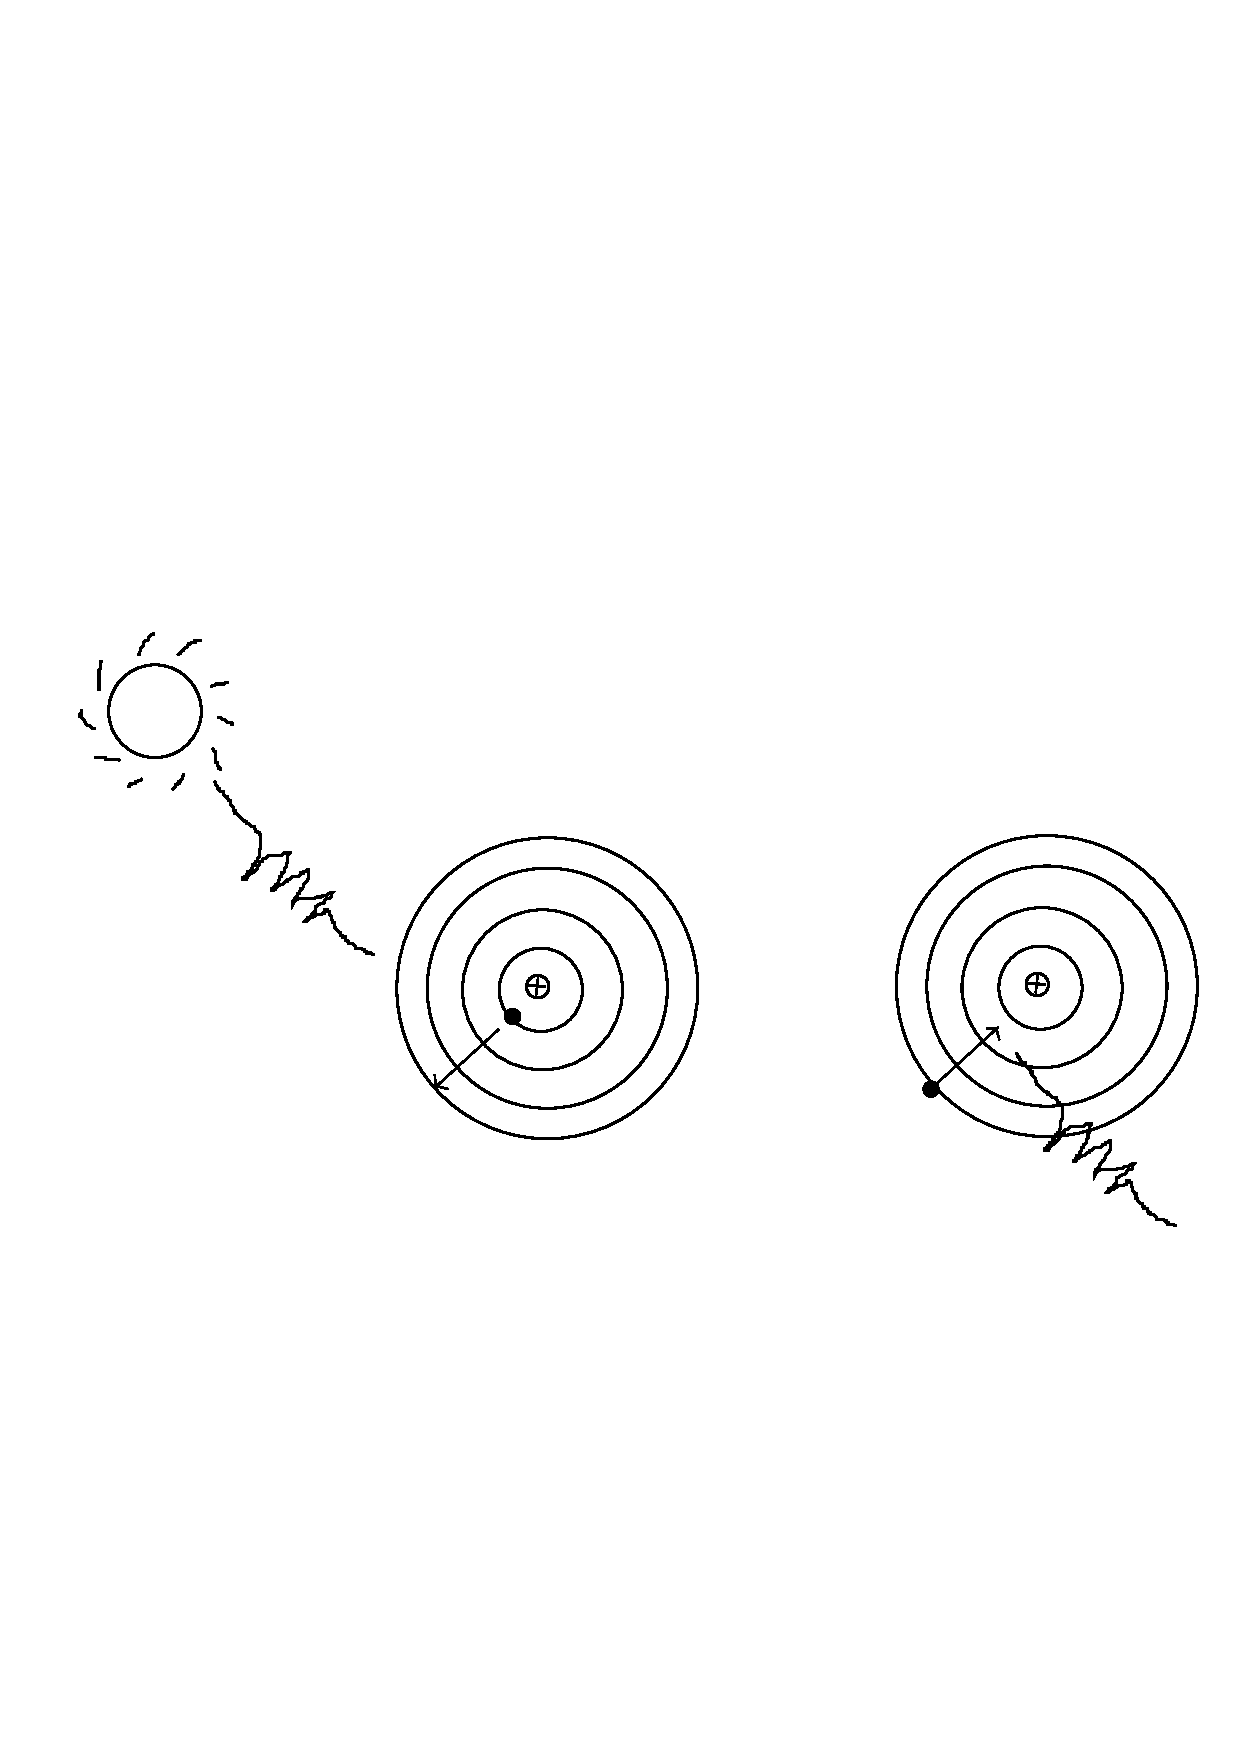
\includegraphics[scale=.5]{untitled.png}
\caption{CIGS electron structure in theory}
\end{figure}


%{\color{red} ???????????????????????????? here I have to insert figure ?????????????????????????????????}

And the main material properties of CIGS and CZTS are summarized as the following table:

%%%%%%%%%%%%%%%%%%%%%%%%table
\begin{table}[H]
\begin{center}
\begin{tabular}{|c|c|c|}
  \hline
  \multicolumn{3}{|c|}{Main properties of CIGS and CZTS} \\
  \hline
   $ $ & CIGS & CZTS \\ \hline
   Absorption coefficient& $10^5$/cm & $10^4$/cm  \\ 
   Band gap& 1.0-1.7 eV & 1.4-1.5 eV   \\ 
   Renewable& In Ga limitation & Abundant   \\ 
   Electron structure& chalcopyrites  & Kesterite and stannite\\ 
   Efficiency in theory& ~26\% & ~30\%   \\ 
   Efficiency in lab& ~20.4\% & ~11.4\%   \\ 
  \hline
\end{tabular}
\caption{}
\end{center}
\end{table}

\section{Basic pricinple of semicondctor}

Here the basic pricinple of semicondctor (Silicon based on doping with Boron and Phosphorous) will be demonstrated in the order of following figures:


\begin{figure}[H]
\centering
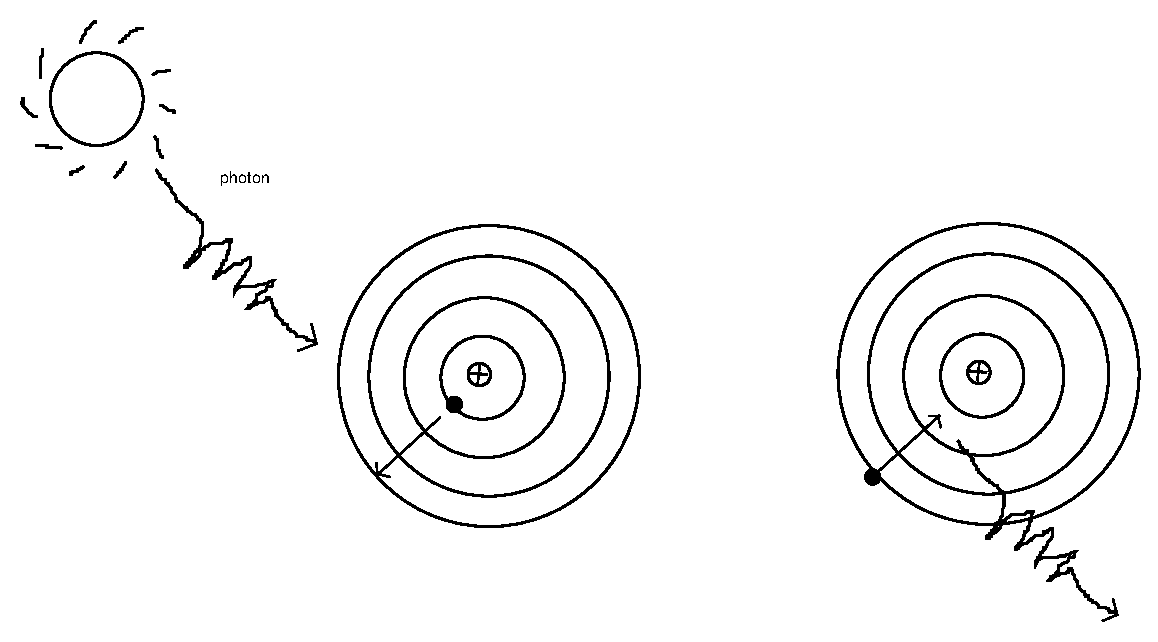
\includegraphics[scale=0.7]{sc1.eps}
\caption{Absorption spectrum}
\label{sc1}
\end{figure}


In the above figure, it shows the relation between sun light and electrons, the electron absorb specified photon energy from sun and is excited 
to higher energy orbit (left figure), and it will jump back as well if the energy is released (right figure) in the Bohr model. One thing needs to be pointed out,
the photon energy has to be some specified energy corresponding to different spectrum in order to let the electron jumps up to higher orbit, which varys according 
to different orbits, and the exact same amount energy will be released if the electron jumps back to ground state. For example, if some light like red color in
the spectrum is absorbed, the electron will be excited from ground state, then one will see the red color when the electron jumps back to ground state. Of course,
the above figure is only intended to illustrate the relation between sun light and electrons, so only one electron is labeled as example.

\begin{figure}[H]
\centering
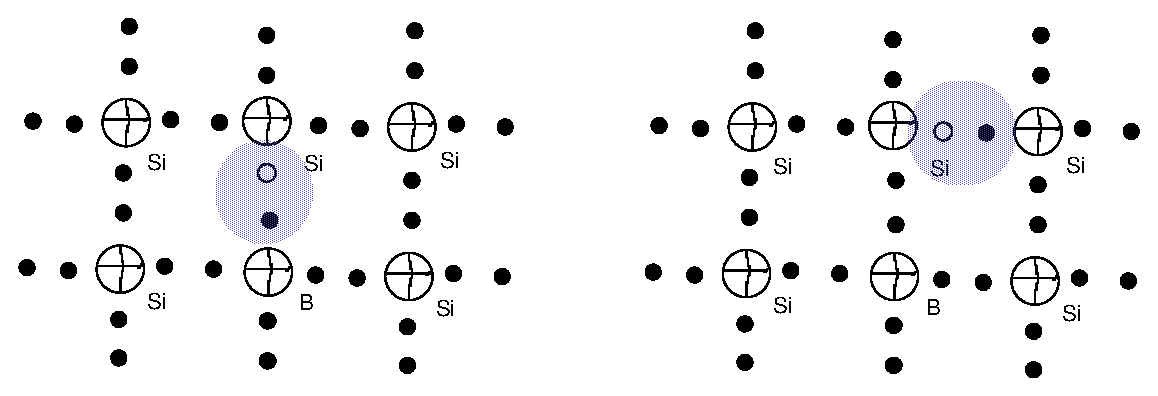
\includegraphics[scale=0.7]{sc2.eps}
\caption{Doping p-type Semiconductor}
\label{sc2}
\end{figure}


where B means the element Boron, which has 3 valence electrons; Si means the element Silicon, which has 4 valence electrons; the black-filled point denotes valence
electron, and free-filled point denotes positive charge hole, when doping one B into the Si semiconductor, there is one positive hole left (left figure), and the
nearby valence electron will shift over to this hole, and instead one hole will show up in another bond (right figure), so the B becomes negative. This is called
p-type doping. Of course, in the real case, there are huge number of doping B, not only one.

\begin{figure}[H]
\centering
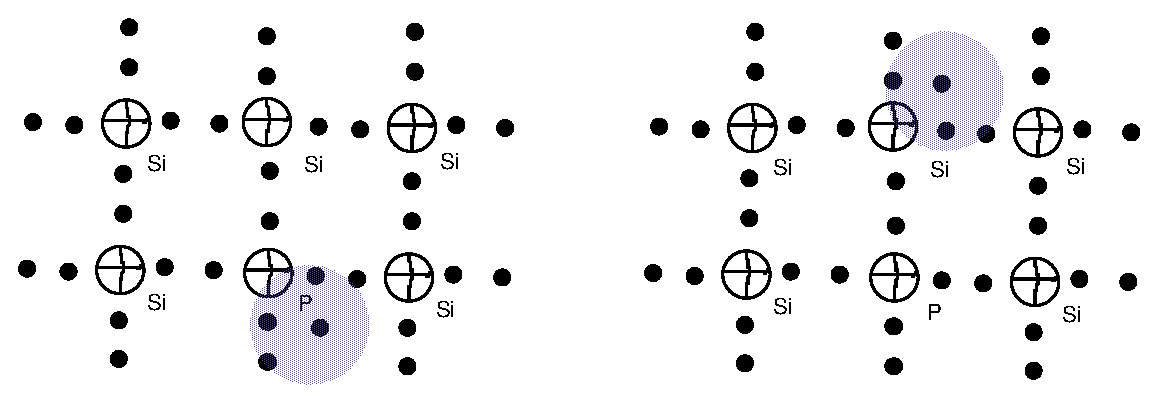
\includegraphics[scale=0.7]{sc3.eps}
\caption{Doping n-type Semiconductor}
\label{sc3}
\end{figure}
 

where P means the element Phosphorous, which has 5 valence electrons. When doping one P into the Si semiconductor, there is one more electron
left for P (left figure), and the electron will move to near Si (right figure), then the P becomes positive. This is called n-type doping. Of course, 
in the real case, there are huge number of doping P, not only one.


\begin{figure}[H]
\centering
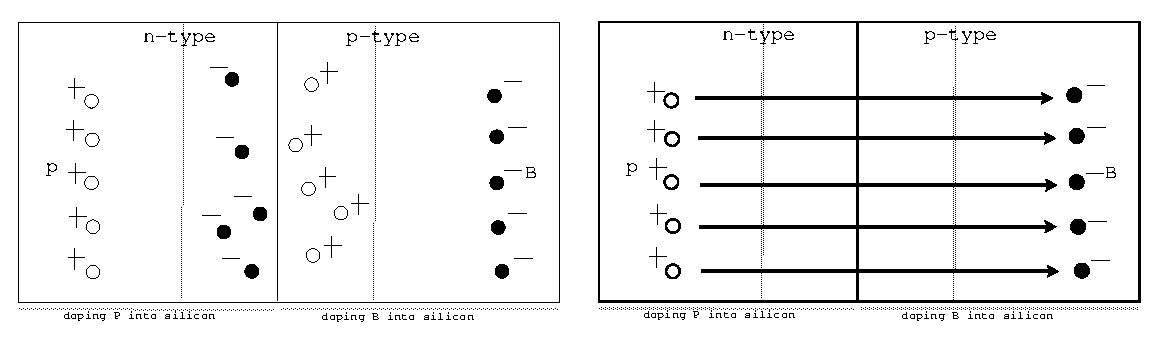
\includegraphics[scale=0.7]{sc4.eps}
\caption{p-n junction (I) }
\label{sc4}
\end{figure}
 
In the above figure, only five doping elements (P and B) are shown to be simplied. So putting p-type and n-type semiconductor together, the p-n junction will be formed.
In the area nearby touching surface (middle area), the electrons and holes will be intended to be paired (left figure), and then one electric field is formed 
(right figure).  

\begin{figure}[H]
\centering
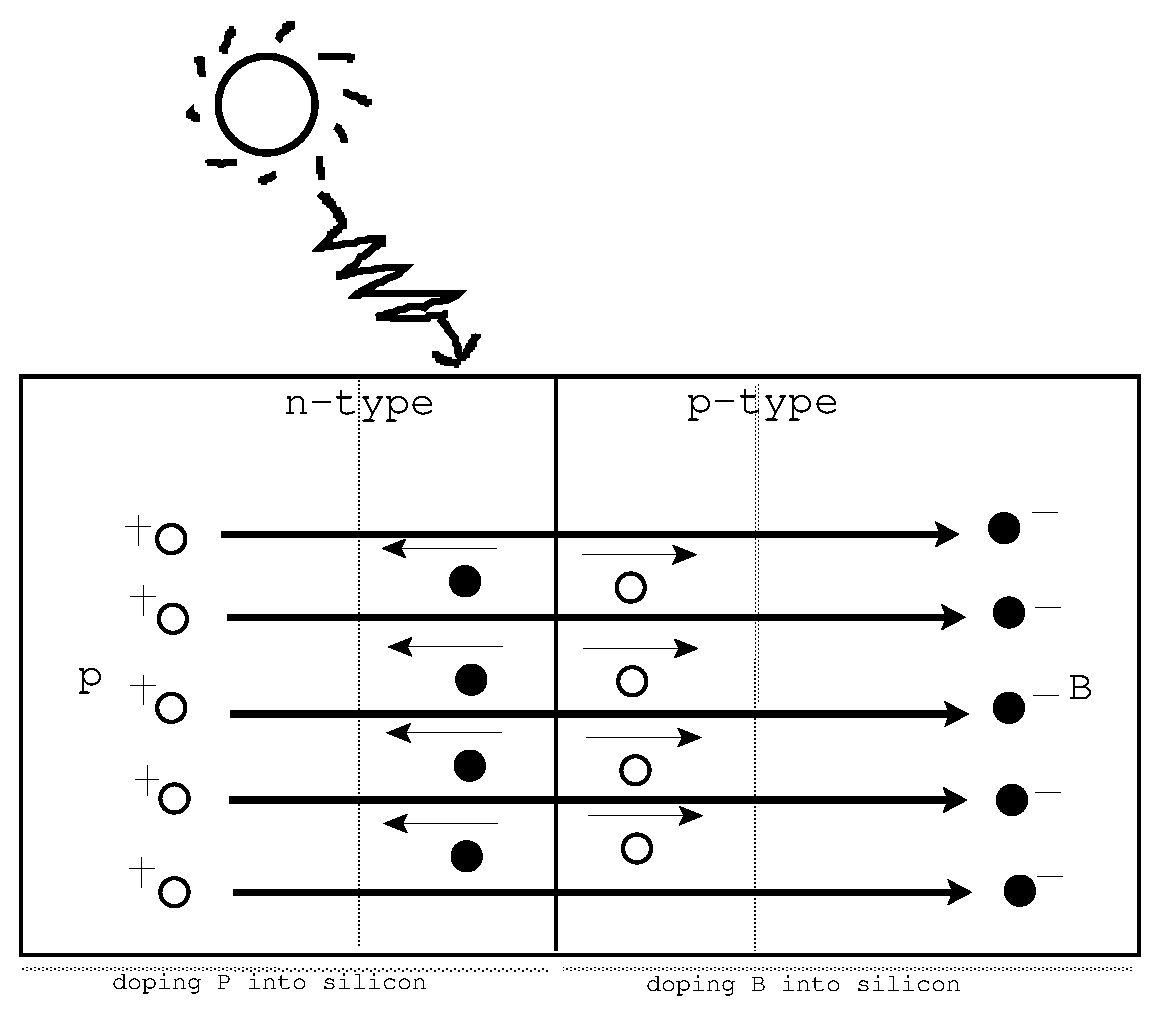
\includegraphics[scale=0.4]{sc5.eps}
\caption{p-n junction (II)}
\label{sc5}
\end{figure}

Now the sun light will excite the equal amount of electrons and holes inside the p-n junction when the light shed on, but they will shift to different direction due
to this electric field.


\begin{figure}[H]
\centering
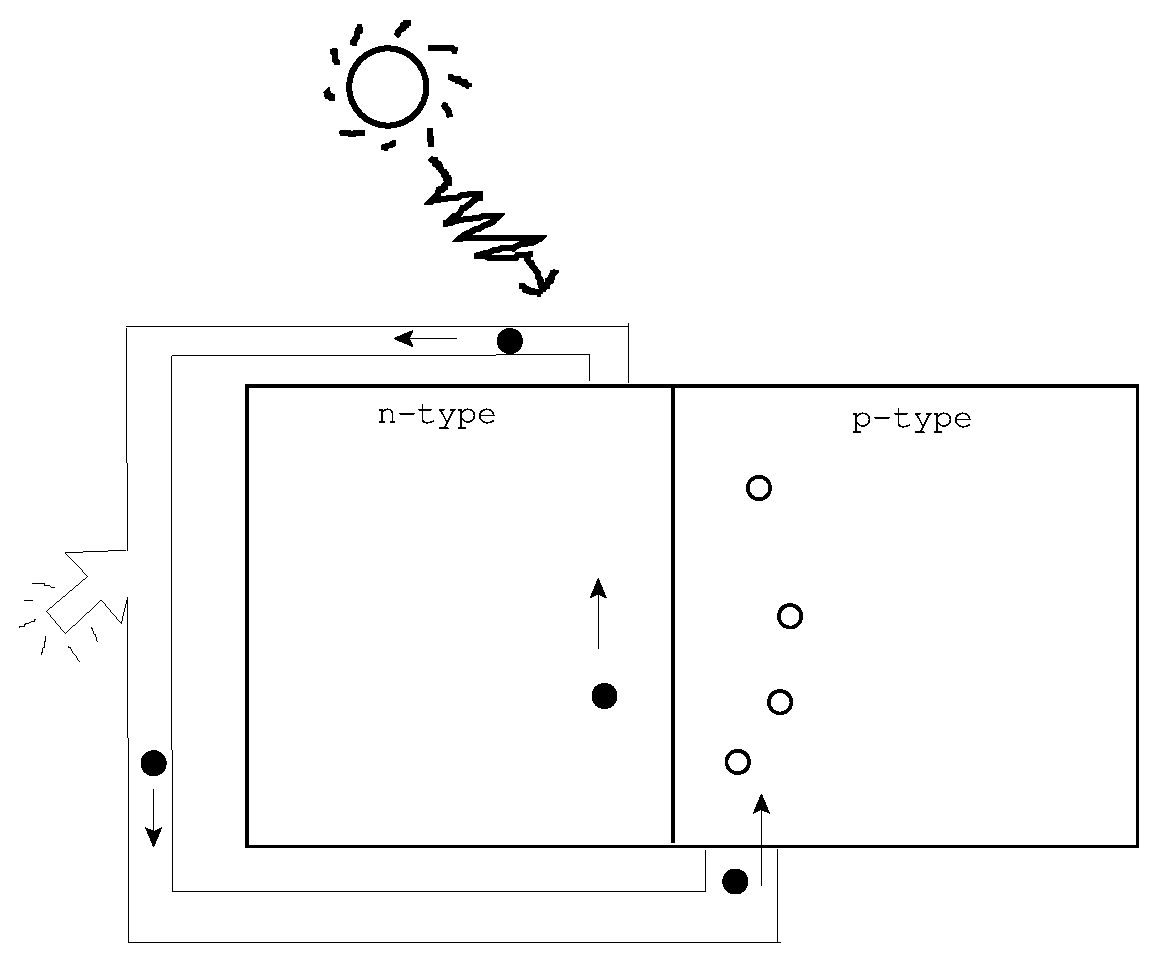
\includegraphics[scale=0.4]{sc6.eps}
\caption{Current}
\label{sc6}
\end{figure}


Finally, when the electric circuit is connected, the electron collected by n-type semiconductor will move through the bulb, and it will be paired after back to p-type semicondctor, and the number of
electrons and holes is the same. If the light shed on continuously, the bulb will light all the time.


\section{Summary}
In this licentiate, the main research material is CIGS, the motivation is that CIGS is a very promising thin film absorber material, although the macroscopic 
properties of CIGS already are farily well understood, there are only little researchs about the details of the electronic energy band dispersion near the uppermost
VBs and CB, which is important for analyzing and understanding electrical properties. So the objective of this licentiate is to improve the parabolic band dispersion
approximation by parametering the band dispersion using the higher order expasion of the traditional k $\cdot$ p method. In this licenciate, the parameterization of
the energy bands for the three uppermost VBs and the lowest CB is presented, and compared with results from the parabolic band approximation and non-parablic band
dispersion. And also, since the low temperature SE study of CIGS is rare, so the ${\varepsilon}$ spectra of CIGS is compared and analysed by experment and theoretical
calculation. 





\chapter{Electronic structure calculations }
\label{ch:dft}

\section{The quantum many-body problem}
\label{ch:mb}

\noindent The solid is a set which includes a huge amount of atoms (around $10^{23}/cm^3$), and the atom is constructed by nuclei and electrons. 
According to the quantum mechanics principles, all the properties of solid matter will be known if one can figure out a way to solve 
the quantum many-body Schrödinger equation exactly. Let us start from the time-independent many-body Schrödinger equation,

 
\begin{equation}\label{ssth}
 {\hath} {\wf} = {E} {\wf}
\end{equation}

\noindent where $\wf$  is the exact wavefunction for the above Schrödinger equation, $\textbf{r}_\textit{i}$ and $\textbf{R}_\textit{I}$  stands for electron and
nucleus coordinators, respectively, $E$ is the energy of the system, $\hath$ is Hamiltonian which has the following form:

\begin{equation}\label{th}
\begin{split}
& \hath = - \sumi<i> {\frac{\hbar^{2}}{2 m_{\textit e}}}   \nablaia<i> - \sumi<I> {\frac{\hbar^{2}}{2 M_\textit{I}}} \nablaia<I>  - \sumij<i><I> \frac{Z_\textit{I}\ e^2}{4 \pi \varepsilon_0 |\textbf{r}_\textit{i}-\textbf{R}_\textit{I}|} \\
& + \frac{1}{2} \suminj<i><j> \frac{ e^2}{4 \pi \varepsilon_0 |\textbf{r}_\textit{i}-\textbf{r}_\textit{j}|} + \frac{1}{2} \suminj<I><J> \frac{Z_\textit{I} Z_\textit{J}\  e^2}{4 \pi \varepsilon_0 |\textbf{R}_\textit{I}-\textbf{R}_\textit{J}|}
\end{split}
\end{equation}


\noindent where the indices $\textit{i}$, $\textit{j}$ are used for electron and $\textit{I}$, $\textit{J}$ are used for atomic nuclei, $Z_\textit{I}$ means the charge of the $\textit{I}$-th nucleus,
here  $\textit{I}$ is a number, and ($\textit{I}$)-th means the ordinal number of $\textit{I}$, $\textit{M}$ denotes nuclear mass, $m_e$ is the electron mass, $\varepsilon_0$ is vacuum permittivity.

\noindent The equation \ref{th} has the following form in atomic units:
\
\begin{equation}\label{sth}\begin{split}
&\hath = - \sumi<i>   \frac{{{\nabla}_{\textit{i}}^{2}}}{2} - \sumi<I> \frac{{{\nabla}_{\textit{I}}^{2}}}{2 M_\textit{I}}  - \sumij<i><I> \frac{Z_\textit{I}}{|\textbf{r}_\textit{i}-\textbf{R}_\textit{I}|} \\
& + \frac{1}{2} \suminj<i><j> \frac{1}{ |\textbf{r}_\textit{i}-\textbf{r}_\textit{j}|} + \frac{1}{2} \suminj<I><J> \frac{Z_\textit{I} Z_\textit{J}\ }{|\textbf{R}_\textit{I}-\textbf{R}_\textit{J}|}
\end{split}\end{equation}


\noindent In equation \ref{sth}, the first and second terms are the kinetic energy operator of the electron and nuclei, respectively,
and the other terms in order are Coulomb interaction between electrons and nuclei, electrons and electrons and nuclei and nuclei.

\noindent Since there are so many atoms to calculate in reality, more importantly, exactly the form of the wavefunction is unknown neither,
so one can not solve the equation \ref{ssth} exactly at present, but people already figure out some ways to approximate the exact solution. 
Generally one can divide these approximations into three different levels, the first level is the Born-Oppenheimer approximation and the second level is Hartree,
Hartree-Fock (HF), density functional theory (DFT) and kohn-sham (KS) equation, the last level is the approximation for solving the secular equation, 
which is an equation that is solved to find the eigenvalue of matrix.

\section{The Born-Oppenheimer approximation}
\label{ch:boa}
\noindent In order to simplify the equation  \ref{ssth}, the first attempt is to seperate the wavefunction of electrons and nuclei, i.e., 
$\wf = {\theta(\textbf{R})} {\Psi(\textbf{r})} $, but since there is a couple term between the electron and nucleus in the Schrödinger Hamitonian in equation \ref{sth}, 
so one can not do that simply. On the other hand, let us observe the equation
\ref{sth} again, there exists a small value ${1}/{M}$, which is part of the nucleus kinetic energy
operator term, the reason is that the mass of nucleus is much larger than that of electron, so if the mass is treated
as infinity, the result is that the electron is seen as interacting under both the external potential caused by nuclei that are fixed in 
some positions and that of other electrons. And a more vividly description is seen from the following figure:
%figure
\begin{figure}[H]
\centering
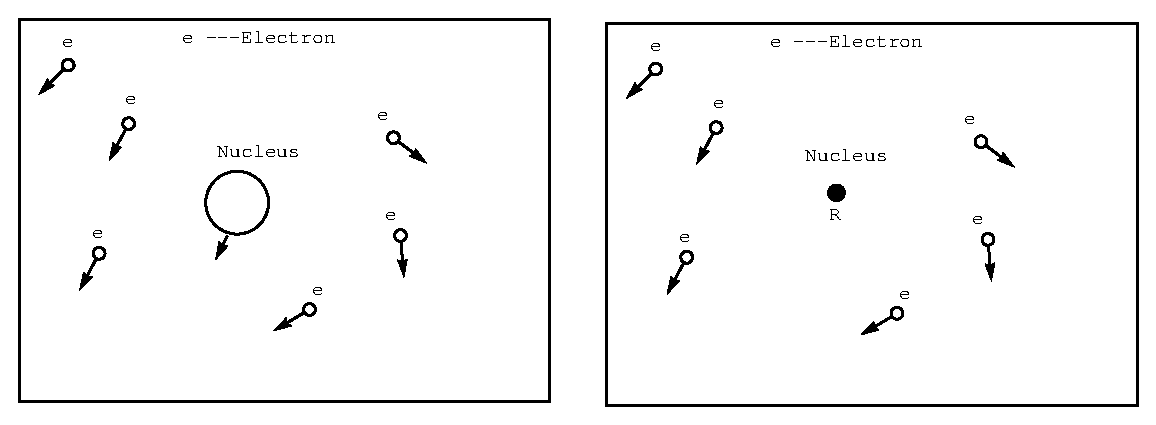
\includegraphics[scale=.5]{system.eps}
\caption{Left one: normal interacting system. Right one. The born-Oppenheimer approximation. The arrow denotes the movement of the nucleus or electron}
\label{fig:bo}
\end{figure}

\noindent The separation of motion between electrons and nuclei is called the Born-Oppenheimer approximation, since the position of nuclei is fixed, so one can define

\begin{equation}\label{nwf}
{\wf}  {\approx}  {\Psi_{ \textit{bo}} ( \{ {\textbf{r}_{\textit{i}}},\textbf{R} \}) } = {\theta(\textbf{R})} {\Psi(\textbf{r}, \textbf{R})}
\end{equation}

 \noindent where $\Psi_{ \textit{bo}} ( \{ {\textbf{r}_{\textit{i}}},\textbf{R} \})$  is the wavefunction of electrons for Born-Oppenheimer approximation, $\textbf R$ is only discrete value belonging to the set of atomic positions, 
 so now, one can recheck the equation \ref{sth} again, one finds out that the term of nuclei kinetic is gone, the term of interacting
 between nuclei is simplified as a constant. Now, the equation \ref{sth} is redefined as follows:

\begin{equation}\label{both}\begin{split}
&{\hath}_\textit{bo}\ =\ - \sumi<i>   \frac{{{\nabla}_{\textit{i}}^{2}}}{2}  - \sumi<i> V_{ext}(\textbf{r}_{\textit{i}})  + \frac{1}{2} \suminj<i><j> \frac{1}{ |\textbf{r}_\textit{i}-\textbf{r}_\textit{j}|} + \frac{1}{2} \suminj<I><J> \frac{Z_\textit{I} Z_\textit{J}\ }{|\textbf{R}_\textit{I}-\textbf{R}_\textit{J}|} \\
&\ = \ \hat{T} \ + \ \hat{V}_\textit{ext} \ + \ \hat{V}_\textit{int}\ + \ N_\textit{II}
\end{split}\end{equation}

\noindent where ${\hath}_\textit{bo}$  is the Hamitonian corresponding the Born-Oppenheimer approximation, the second term is the nuclei potential acting on the
electrons, 

\begin{equation}
V_{ext}(\textbf{r}_{\textit{i}}) =  \sumi<I> \frac{Z_\textit{I}}{|\textbf{r}_\textit{i}-\textbf{R}_\textit{I}|}
\end{equation}

\noindent where the subscript $ext$ in the second term means $external$, so this term is about external potentials interaction. 
The corresponding Schrödinger equation is:

\begin{equation}\label{bose}
{\hath}_{bo} \wfbo = E_\textit{bo} {\wfbo}
\end{equation}

\noindent where $E_\textit{bo}$ is the energy of this electronic system. So far,
the discussion above is only considering the Schrödinger equation of electron, i.e., equation \ref{bose}, so how about the Schrödinger equation of nucleus? First, comparing equation
\ref{sth} and \ref{both}, the total Schrödinger Hamitonian can be rewritten as: 

\begin{equation}\label{nh}
 {\hath} = - \sumi<I> \frac{{{\nabla}_{\textit{I}}^{2}}}{2 M_\textit{I}} + {\hath}_{bo}
\end{equation}

\noindent so the new Schrödinger equation with equation \ref{nh} and \ref{nwf} is 

\begin{equation}
 (- \sumi<I> \frac{{{\nabla}_{\textit{I}}^{2}}}{2 M_\textit{I}} + {\hath}_{bo} ) ( {\theta(\textbf{R})} {\Psi(\textbf{r}, \textbf{R})}) = E_{m}({\textbf R}) ({\theta(\textbf{R})} {\Psi(\textbf{r}, \textbf{R})} )
\end{equation}
 
\noindent where $E_{m}$ is the total energy of above system, after some steps of derivation, one can end up with the following equation:
\begin{equation}\label{ise}
( \hat{H}_{I1}+\hat{H}_{I2}+\hat{H}_{I3}+E_{bo}({\textbf R}) ) {\theta(\textbf{R})} = {E_m} {\theta(\textbf{R})}
\end{equation}

\noindent where

\begin{equation}\begin{split}
 &  \hat{H}_{I1} = - \sumi<I> \frac{{{\nabla}_{\textit{I}}^{2}}}{2 M_\textit{I}}   \\
 &  \hat{H}_{I2} = - \sumi<I> \frac{1}{M_\textit{I}} {\int {\Psi(\textbf{r}, \textbf{R})}^{\ast} {{\nabla}_{\textit{I}}} {\Psi(\textbf{r}, \textbf{R})} d {\textbf r }} {{\nabla}_{\textit{I}}} \\
 &  \hat{H}_{I3} = - \sumi<I> \frac{1}{M_\textit{I}} {\int {\Psi(\textbf{r}, \textbf{R})}^{\ast} {{\nabla}_{\textit{I}}^{2}} {\Psi(\textbf{r}, \textbf{R})} d {\textbf r }} 
\end{split}\end{equation}

\noindent from equation \ref{ise}, one obseves that the lattice dynamical properties of certain system within the Born-Oppenheimer approximation could be obtained, and in this equation,
the gournd state energy $E_{bo}({\textbf R})$ of electron system is needed to solve equation \ref{ise}, here $\textbf R$ is the parametrilized value from the atom position.
 

\noindent In summary, the Schrödinger equation of electron and nucleus is derived seperatly in this section, and usually, when one refers to calculate the ground state properties,
which means to take use of the Schrödinger equation of electron only, e.g., equation \ref{bose}, and Schrödinger equation of nucleus is used for the calculation of lattice dynamics.

So far, one notices that the equation \ref{both} is much simpler than equation \ref{sth}, but still not solvable, so further more excellent approximations  are needed
to solve this many-body problem.


\section{Hartree and Hartree-Fock approximation}
\noindent Hartree or Hartree-Fock method is straightforward to get the 
expression using the mathematical approaches, and both of them focus on the treatment of wavefunction, however, the wavefunction in Hartree method is not 
flexible enough, and better but not enough (lacking of correlation term) in Hartree Fock method.

%the density functional theory (DFT) is a perfect method which can solve the 
%many-body equation in theory, but not solvable in practice

\subsection{Hartree approximation}
\label{ha}
\noindent The simplest approximation of the wavefunction for many-body Schrödinger equation is the form of acting like non-interacting 
electrons, so the wavefunction with N non-interacting electrons has the following expression:

\begin{equation}\label{wfh}
\wfh = \bwf<1><1> \bwf<2><2> \cdots \bwf<N><N> 
\end{equation}

\begin{comment}
\begin{equation}\label{wfh}
\langle \rangle
\end{equation}
\end{comment}


\noindent where $i$ goes through all the electrons, and  means state of the $i$-th electron in the position of ${\textbf{r}}_{\textit{i}}$, 
from here and following the $R$ is suppressed in the wavefunction since they are position fixed. So the total energy of the system can be written down 
in the following way :

\begin{equation}\label{teh}
E_{\textit{h}} = <\wfh |\ {\hath}_{\textit{bo}} \ | \wfh  >
\end{equation}

\noindent So making the substitution using equation \ref{both} and \ref{wfh} into equation \ref{teh}, so the total energy of system is:
\begin{equation}\begin{split}
&E_\textit{h} = \sumi<i> <\bwf<i><> |\ -\frac{\nabla^{2}_{\textit r}}{2} + V_\textit{ext}(\textbf{r})  \ | \bwf<i><> > \\
& +\frac{1}{2} \suminj<i><j> <\bwf<i><> \bwfn<j><'>|\ \frac{1}{|\textbf{r} - \textbf{r}^{'} |} \ | \bwf<i><> \bwfn<j><'>>
\end{split}\end{equation}

\noindent In order to calculate the stationary state of the system, so the variation of the wavefunction should be
zero variation in the energy, so here one can set up the following equation with Lagrange multiplier $E^{i}_h$
\begin{equation}\label{haa}
 \delta [ E_{\textit{h}} - \sumi<i> E^{i}_{h} (<\bwf<i><> | \bwf<i><> > -1)] = 0 
\end{equation}

\noindent In order to calculate the term $\delta ( E_{\textit{h}} ) $, one has to know
\begin{equation}\begin{split}\label{hartree1}
& \delta ( \sumi<i> <\bwf<i><> |\ -\frac{\nabla^{2}_{\textbf r}}{2} + V_\textit{ext}(\textbf{r})  \ | \bwf<i><> > ) \\
&  = \sumi<i> \{ < \delta \bwf<i><> |\ -\frac{\nabla^{2}_{\textbf r}}{2} + V_\textit{ext}(\textbf{r})  \ | \bwf<i><> >  \\
&  + <  \delta \bwf<i><> |\ -\frac{\nabla^{2}_{\textbf r}}{2} + V_\textit{ext}(\textbf{r})  \ |  \bwf<i><> >^{\ast} \}
\end{split}\end{equation}

\noindent and 

\begin{equation}\begin{split}\label{hartree2}
&  \delta( \frac{1}{2} \suminj<i><j> <\bwf<i><> \bwfn<j><'>|\ \frac{1}{|\textbf{r} - \textbf{r}^{'} |} \ | \bwf<i><> \bwfn<j><'>>)   \\
& =   \frac{1}{2} \suminj<i><j> \{  <\delta \bwf<i><> \bwfn<j><'>|\ \frac{1}{|\textbf{r} - \textbf{r}^{'} |} \ | \bwf<i><> \bwfn<j><'>>  \\
& +   < \bwf<i><> \delta \bwfn<j><'>|\ \frac{1}{|\textbf{r} - \textbf{r}^{'} |} \ | \bwf<i><> \bwfn<j><'>> +  T_{rem}\}
\end{split}\end{equation}

\noindent where $T_{rem}$ is the remaining terms, actually these remaining terms will not affect the derivation. Before getting the final result, 
there is one more identity 

\begin{equation}\begin{split}\label{hartreelabel1}
& < \bwf<i><> \delta \bwfn<j><'>|\ \frac{1}{|\textbf{r} - \textbf{r}^{'} |} \ | \bwf<i><> \bwfn<j><'>> \\
& = \int d \textbf{r} d \textbf{r}{'}  \phi_{i}^{*} (\textbf{r}{}) \delta \phi_{j}^{*} (\textbf{r}{'}) \frac{1}{|\textbf{r} - \textbf{r}^{'} |}  \phi_{i}^{} (\textbf{r}{})  \phi_{j}^{} (\textbf{r}{'})\\
& = \int d \textbf{r}{'} d \textbf{r}  \phi_{i}^{*} (\textbf{r}{'}) \delta \phi_{j}^{*} (\textbf{r}{}) \frac{1}{|\textbf{r}{'} - \textbf{r} |}  \phi_{i}^{} (\textbf{r}{'})  \phi_{j}^{} (\textbf{r})\\
& = <\delta \bwf<j><> \bwfn<i><'>|\ \frac{1}{|\textbf{r} - \textbf{r}^{'} |} \ | \bwf<j><> \bwfn<i><'>>
\end{split}\end{equation}

\noindent So the equation \ref{hartree2} will become 

\begin{equation}\begin{split}\label{hartree3}
&  \delta( \frac{1}{2} \suminj<i><j> <\bwf<i><> \bwfn<j><'>|\ \frac{1}{|\textbf{r} - \textbf{r}^{'} |} \ | \bwf<i><> \bwfn<j><'>>)   \\
& =  \suminj<i><j> \{  <\delta \bwf<i><> \bwfn<j><'>|\ \frac{1}{|\textbf{r} - \textbf{r}^{'} |} \ | \bwf<i><> \bwfn<j><'>> + \frac{T_{rem}}{2}\}
\end{split}\end{equation}


Taking use of the above two equation \ref{haa}, \ref{hartree1}, \ref{hartree3} and variation in the term of  $\delta \phi^{*}_{i}(\textbf{r}{}) $,
finally it ends up with
\begin{equation}\label{hha}
(-\frac{\nabla^{2}_{\textbf r}}{2} + V_\textit{ext}(\textbf{r})+ \suminj<j><i> <\bwfn<j><'>\ | \frac{1}{|\textbf{r} - \textbf{r}^{'} |} \ | \bwfn<j><'>>) \bwf<i><> = E^{i}_{h} \bwf<i><>
\end{equation}
\noindent where $E^{i}_{h}$  also can be treated as the energy corresponding the ($i$)-th electron in the position of  $\textbf{r}$, the equation \ref{hha} is a group of dependent single
 particle equations, and after checking it, one will find out which is an equation that is self-consistent and can be solved using computer by iteratively.


%%%%%%%%%%%%%%%%%%%%figure
\begin{comment}
\noindent where $\wfhit<0>$ is the initial wavefunction,$\wfhit<m+1>$ and $\wfhit<m>$ are the wavefunction of ($m$)-th the ($m+1$)-th iteration solving the Hartree equation,
 respectively, and $\delta$ is the tolerance.
\end{comment}

\subsection{Hartree-Fock approximation}
\noindent Hartree approximation is the lowest level approximation, and Hartree-Fock approximation is the method which considers the 
antisymmetry of the wavefunction, which means that if the positions of two electrons (with same spin) are exchanged, the wave 
function should change the sign, like:
\begin{equation}\label{hfwf}
\Psi_\textit{hf} (\{ \cdots \textbf{r}_\textit{i} \cdots  \textbf{r}_\textit{j} \}) = - \Psi_\textit{hf} (\{ \cdots \textbf{r}_\textit{j} \cdots  \textbf{r}_\textit{i} \})
\end{equation}
\noindent Slater introduced  an excellent way to construct the wavefunction due to the equation \ref{hfwf} based on the Hartree approximation, 
the wavefunction of many- body Schrödinger equation is written down  in a matrix determinant way for the number of $N$ electrons 
(without spin):
\begin{equation}\label{hfwfm}
\Psi_{hf}(\mathbf{r}_1, \mathbf{r}_2, \ldots, \mathbf{r}_N) =
\frac{1}{\sqrt{N!}} \left|
\begin{matrix}
    \bwf<1><1> & \bwf<1><2> & \cdots & \bwf<1><N> \\
    \bwf<2><1> & \bwf<1><2> & \cdots & \bwf<1><N> \\
    \vdots               & \vdots               &        & \vdots               \\
    \bwf<N><1> & \bwf<N><2> & \cdots & \bwf<N><N>
\end{matrix} \right|
\end{equation}
\noindent where $i$ goes through all the electron, and $\bwf<i><i>$ means state of the ($i$)-th electron in the position of $\textbf{r}_\textit{i}$, so if one exchanges two rows
 in the equation \ref{hfwfm}, the result is satisfied with the equation \ref{hfwf}.

\noindent Now repeating all the processes already done through the Hartree approximation, the total energy of Hartree-Fock is as follows:

\begin{equation}\begin{split}
&E_\textit{hf} = \sumi<i> <\bwf<i><> |\ -\frac{\nabla^{2}_{\textit r}}{2} + V_\textit{ext}(\textbf{r})  \ | \bwf<i><> > \\
& + \frac{1}{2} \suminj<i><j> <\bwf<i><> \bwfn<j><'>|\ \frac{1}{|\textbf{r} - \textbf{r}^{'} |} \ | \bwf<i><> \bwfn<j><'>> \\
& - \frac{1}{2} \suminj<i><j> <\bwfn<i><'> \bwfn<j><>|\ \frac{1}{|\textbf{r} - \textbf{r}^{'} |} \ | \bwfn<i><> \bwfn<j><'>>
\end{split}\end{equation}

\noindent In the same mathematical skill but more complicated like in previous section, the dependent singe particle Hartree-Fock equation can be obtained:

\begin{equation}\begin{split}
& \{ -\frac{\nabla^{2}_{\textit i}}{2} + V_\textit{ext}(\textbf{r})+ \suminj<j><i> <\bwfn<j><'>\ | \frac{1}{|\textbf{r} - \textbf{r}^{'} |} \ | \bwfn<j><'>> \} \bwf<i><>  \\
& - \suminj<i><j>  < \bwfn<j><'>|\ \frac{1}{|\textbf{r} - \textbf{r}^{'} |} \ | \bwfn<i><'> >) \bwfn<j><>  = E^{i}_{hf} \bwf<i><>
\end{split}\end{equation}

\noindent Comparing with Hartree equation, there is an extra term in the equation above, which is called exchange term, and at the same time,
 in order to organize the equation in a nice and clear way, finally it ends up with:
\begin{equation}\begin{split}
\{ -\frac{\nabla^{2}_{\textit i}}{2} + V_\textit{ext}(\textbf{r}) +V_\textit{H}(\textbf{r}) \}  \bwf<i><>  = E^{i}_{hf}   \bwf<i><> 
\end{split}\end{equation}
where
\begin{equation}
 V_\textit{H}(\textbf{r})= \int \frac{\rho(\textbf{r}{'}) - \rho_{\textit{i}}^{\textit{HF}}(\textbf{r},\textbf{r}{'})}{|\textbf{r} - \textbf{r}^{'} |}  \mathrm{d}\textbf{r}^{'}
\end{equation}
and $ \rho_{\textit{i}}^{\textit{HF}}(\textbf{r},\textbf{r}{'}) = \sumi<j> \frac{\phi_{i}^{}(\textbf{r}{'}) \phi_{i}^{*}(\textbf{r}{}) \phi_{j}^{}(\textbf{r}{}) \phi_{j}^{*}(\textbf{r}{'})} {\phi_{i}^{}(\textbf{r}) \phi_{i}^{*}(\textbf{r})} $ 
; $\rho(\textbf{r}) = \sumi<i>  {|\bwf<i><>|}^{2}$ . And also it could be solved in the same way like Hartree approximation but plus one extra term.

\section{Density functional theory}
\noindent Hartree and Hartree-Fock methods are very classic methods to solve many-body Schrödinger equation. However, HF method only includes the exchange,
 but badly in the electron correlation, so they are not suitable in the case of electrons in solid. Apart from the two methods mentioned before, there is another modern method to deal with
 the more complicated calculation of electrons, namely, density functional theory (DFT), which is introduced by Hohenberg and
 Kohn in 1964, Kohn and Pople was awarded by Chemistry Nobel Prize in 1998.

\noindent The idea of this method is to treat the electron density of solid instead of using the many-particle wavefunction, so one can
 benefit that the degree of freedom reduces from 3N (N is the number of electrons) to 3, which is apparently less complicate than 
those of Hartree and Hartree-Fock during calculation. 

\subsection{The Density as Basic Variable}
\noindent There are two questions coming out if considering the electron density as the role of wavefunction. The first one is whether it
 is the equivalence relation between the electron density and wavefunction of the system, and the second one is how to solve this 
problem. In order to know that there are two very basic theorems introduced by Hohenberg and Kohn:

\begin{thm}
\label{hk1}
\noindent The first theorem says that the external potential $V_\textit{ext}(\textbf{r})$  is determined uniquely for any of electon system by the ground state electron density $\rho_0$.
\end{thm}

\noindent The above theorem also indicate that all the ground state properties are decided by the true ground state density $\rho_0$,
for example, the total energy E=E[$\rho_0$]. 
\noindent The above theorem also explains the equivalence relation between the electron density and wavefunction, because Hamiltonian is obtained from external potentials,
then one can get the wavefunction, so the corresponding electron density is determined, however, from the theorem, the external potential is unique decided by electron
density, so the electron density contains the same information of wavefunction.

\noindent The proof of theorem is following:

\noindent Now, let us assume that there exsits two external potentials named $V^{1}_\textit{ext}(\textbf{r})$ and $V^{2}_\textit{ext}(\textbf{r})$ leading to the same ground state 
electron density $\rho_0$, but obviously, which will lead to two different Hamiltonians, that is, $\hat{H}_{1}$ and $\hat{H}_{2}$, and as well as two different corresponding
wavefunctions named $\Psi_1$ and $\Psi_2$. Since $\Psi_1$ are not the ground state wavefunction of $\hat{H}_{2}$, the same rules to $\Psi_2$ and $\hat{H}_{1}$, so two following
inequality equations will be satisfied:

\begin{equation}\label{hkpf1}\begin{split}
&  E_1 = \langle \Psi_1\ |\hat{H}_{1}|\ \Psi_1 \rangle  \ < \  \langle \Psi_2\ |\hat{H}_{1}|\ \Psi_2 \rangle\\
&  E_2 = \langle \Psi_2\ |\hat{H}_{2}|\ \Psi_2 \rangle  \ < \  \langle \Psi_1\ |\hat{H}_{2}|\ \Psi_1 \rangle
\end{split}\end{equation}

\noindent Taking advangtage of the form of Hamitonian from equation \ref{both}, one can get:
\begin{equation}\label{hkpf2}\begin{split}
&    \langle \Psi_2\ |\hat{H}_{1}|\ \Psi_2 \rangle \\
&  = \langle \Psi_2\ |\hat{H}_{2} + \hat{H}_{1} - \hat{H}_{2}|\ \Psi_2 \rangle \\
&  = \langle \Psi_2\ |\hat{H}_{2} |\Psi_2 \rangle + \langle \Psi_2 | \hat{H}_{1} - \hat{H}_{2}|\ \Psi_2 \rangle \\
&  = E_2 + \int d \textbf{r} ( V^{1}_\textit{ext}(\textbf{r}) - V^{2}_\textit{ext}(\textbf{r}) )  \rho_0
\end{split}\end{equation}

\noindent So using \ref{hkpf1} and \ref{hkpf2}, one can get:

\begin{equation}\label{hkpf3}
 E_1  < \  E_2 + \int d \textbf{r} ( V^{1}_\textit{ext}(\textbf{r}) - V^{2}_\textit{ext}(\textbf{r}) )  \rho_0
\end{equation}

\noindent Another similar inequality equation will be gained if one changes the form of equation $\langle \Psi_1\ |\hat{H}_{2}|\ \Psi_1 \rangle$ like equation \ref{hkpf2}.
\begin{equation}\label{hkpf4}
  E_2  < \  E_1 + \int d \textbf{r} ( V^{2}_\textit{ext}(\textbf{r}) - V^{1}_\textit{ext}(\textbf{r}) )  \rho_0
\end{equation}

\noindent so plus the left and right sides from equation \ref{hkpf3} and \ref{hkpf4}, one will gain a contradictory result:
\begin{equation}\label{hkpf4}
  E_1 + E_2  < \  E_2 + E_1
\end{equation}

\noindent So the external potential $V_\textit{ext}(\textbf{r})$ is unique.

\begin{thm}
\label{hk2}
\noindent The second theorem says that there is a universal functional for the total energy in the terms of the electron density $\rho$ with any external potential $V_\textit{ext}(\textbf{r})$ ,
and the exact ground state density is gained when the ground state total energy functional reaches its minimal value, that is, E[$\rho$]>E[$\rho_0$], where $\rho$ is not the ground state density.
\end{thm}

\noindent The proof of theorem is following:
Because of the first theorem, so the total energy can be expressed in the following way (ignoring the interaction between nuclei):
\begin{equation}\label{hkpf5}\begin{split}
& E[\rho] \ =\langle \Psi  | \ \hat{T} \ + \ \hat{V}_\textit{int}  \ + \ \hat{V}_\textit{ext} \ | \Psi \rangle \\
&     = \langle \Psi  | \ \hat{V}_\textit{ext} \ | \Psi \rangle  + \underbrace{\langle \Psi  | \ \hat{T} \ + \ \hat{V}_\textit{int}  \ \ | \Psi \rangle}  \\
&     =   \ \int \rho(\textbf{r}) V_\textit{ext}  + \                    F[\rho] 
\end{split}
\end{equation}

\noindent In the above equation \ref{hkpf5}, the term of $F[\rho]$ is the universal functional since all the systems of electrons.

\noindent Now, let us say $\rho_0$ is the exact ground state electron density, from first theorem, there exists one unique external potential $V_\textit{ext}$, so 
the corresponding Hamitonian and wavefunction are $\hat{H}$ and $\Psi_0$, assuming that a different electron density $\rho$ which is not exact ground state density 
corresponding to the wavefunction $\Psi_0$, then one will get:

\begin{equation}
E[\rho_0] = \langle \Psi_0\ |\hat{H}|\ \Psi_0 \rangle 
          < \langle \Psi\ |\hat{H}|\ \Psi \rangle \
          = E[\rho]
\end{equation}

\noindent so from above equation, one knows the total energy for the case of exact ground state electron density is lower than any other cases, which also means that one can get 
the exact ground state electron density by minimizing the total energy.



\noindent From those two theorems, one definitely know how to solve this problem theoretically, but in practice, $E[\rho]$ is unknown how it looks like, 
so one more method is needed to deal with it, namely, Kohn-Sham (KS) equation.

\section{The Kohn-Sham equation}

\noindent Since I already introduced the Hartree and Hartree Fock method to solve the many-body problem, both of which are based on the idea which is to transform complex 
many-body problem to single particle problem by using wavefunction, but Density functional theory only consider to take use of information from Hamitonian, but not solvable, 
so is it possbile to combine these two ideas together? the answer is yes,the DFT is solved by Kohn-Sham equation introduced by Kohn and Sham in 1965,
which I recommended a way to construct in the following text (ignoring the interaction between nuclei)

\noindent First of all, the total energy can be expressed by the following:
\begin{equation}
\label{kse}
\begin{split}
&E[\rho] \ =\ T[\rho] \ + \ V_\textit{int}[\rho] \ + \ V_\textit{ext}[\rho]  \\
&\ \ \   = \underbrace{\ (T[\rho] \ - \ T_{0}[\rho]) \ + \  (V_\textit{int}[\rho] \ - \ V_\textit{HF}[\rho])\ }+ \ T_{0}[\rho] \ + \ V_\textit{HF}[\rho] \ + V_\textit{ext}[\rho]       \\
&\ \ \   = \ T_{0}[\rho] \ + \ V_\textit{HF}[\rho] \ + \ V_\textit{C}[\rho] +\ V_\textit{ext}[\rho]
\end{split}
\end{equation}
\noindent where $E[\rho]$  is the total energy, $\rho$ is the ground state density;$V_\textit{int}[\rho]$, $T[\rho]$ and $V_\textit{int}[\rho]$ are the energy from external potential, the exact kinetic 
and the exact electron-electron potential energy; $T_{0}[\rho]$ is the kinetic energy of a non-interacting electrons, $V_\textit{HF}[\rho]$ is the potential  from Hartree-Fock approximation.

\noindent From the Hartree-Fock approximation, one can further know that:
\begin{equation}
 V_\textit{HF}[\rho] \ = \ V_\textit{H}[\rho] \ + \ V_\textit{X}[\rho] 
\end{equation}

\noindent where $V_\textit{H}[\rho]$ and $ V_\textit{X}[\rho] $ are the Hartree contribution and exchange contribution, respectively, so the equation (13) can be further defined like
 the following:
\begin{equation}\label{ccc}
\begin{split}
&E[\rho]\ = \ T_{0}[\rho] \ + \ V_\textit{H}[\rho] \ + \ V_\textit{ext}[\rho] \ + \ \underbrace{\ V_\textit{X}[\rho]  \ + \ V_\textit{C}[\rho]}  \\
&\ \ \ = \ T_{0}[\rho] \ + \ V_\textit{H}[\rho] \ + \ V_\textit{ext}[\rho] + \ V_\textit{XC}[\rho]
\end{split}\end{equation}
\noindent where $V_\textit{XC}[\rho]$  is the exchange-correlation term. From equation \ref{kse}, the explicit expression of $V_\textit{XC}[\rho]$ one does not know. 
 but the first three terms one already know

\begin{equation}
 T_{0}[\rho]\ = \ < \Psi_{i}(\textbf{r}) \ | -\frac{\nabla^{2}_{r}}{2} \ | \Psi_{i}(\textbf{r}) >
\end{equation}

\begin{equation}
V_\textit{H}[\rho] \ = \ \frac{1}{2} \int \int \mathrm{d} {\textbf{r}} \mathrm{d}{\textbf{r}^{\prime}} \frac{\rho({\textbf{r}})\rho(\textbf{r}^{\prime})}{|{\textbf{r}}-{\textbf{r}}^{\prime}|} 
\end{equation}


\begin{equation}
V_\textit{ext}[\rho]\ = \ \int \mathrm{d}{\textbf{r}} \rho(\textbf{r}) V_\textit{ext} 
\end{equation}

\noindent In order to derive the ground state of the above system, one can view this problem as the process of minimizing the total energy by varying the wavefunction $\Psi^*$, since
 the wavefunction can be constructed to electron density (equation \ref{ks1}), just like the derivation in the section of Hartree, finally one can get the Kohn-Sham equation.
\begin{equation}\label{aaa}
 (-\frac{\nabla^{2}_{r}}{2}\ + \ V_\textit{KS}) \Psi_{\textit{i}}(\textbf{r}) = E_{\textit{ks}}^{\textit{i}} \Psi_{\textit{i}}(\textbf{r})
\end{equation}

\noindent where
\begin{equation}\begin{split}
&\ V_\textit{KS} \ = \ V_\textit{ext}[\rho] + \int \frac{\rho(\textbf{r}^{\prime})}{|{\textbf{r}}-{\textbf{r}}^{\prime}|} \ + \ \frac{\delta{E_\textit{XC}}}{\delta{\rho(\textbf{r})}} \\
&\ = \ \ V_\textit{ext}[\rho] + \int \frac{\rho(\textbf{r}^{\prime})}{|{\textbf{r}}-{\textbf{r}}^{\prime}|} \ + \ \upsilon_\textit{xc}
\end{split}
\end{equation}

\noindent One can think of the Hamiltonian in another point of view, e.g., single particle system with three different potentials. Now the
 problem turns out to be like the single particle form with the degree of freedom of 3.

\noindent So the many-body problem now is transformed to the single electron problem, if the $\upsilon_\textit{xc}$  is exact, the exact ground-state density is :
\begin{equation}\label{ks1}
 \rho(\textbf{r}) = \sumi<i> {\Psi^{*}_{i}(\textbf{r})} {\Psi_{i}(\textbf{r})}
\end{equation}

\noindent There is no total energy equation expression yet, however, if one can change the equation \ref{aaa} as 
\begin{equation}\label{bbb}
\sumi<i> \Psi^{*}_{\textit{i}}(\textbf{r})(-\frac{\nabla^{2}_{i}}{2}\ + \ V_\textit{KS}) \Psi_{\textit{i}}(\textbf{r}) = \sumi<i> \Psi^{*}_{\textit{i}}E_{\textit{ks}}^{\textit{i}} \Psi_{\textit{i}}(\textbf{r})
\end{equation}

\noindent Based on equation \ref{ccc} and \ref{bbb}, the total energy expression is:
\begin{equation}\label{totalenergy}
\begin{split}
& E= \sumi<i> E_{\textit{ks}}^{\textit{i}} - \ \frac{1}{2} \int \int \mathrm{d} {\textbf{r}} \mathrm{d}{\textbf{r}^{\prime}} \frac{\rho({\textbf{r}})\rho(\textbf{r}^{\prime})}{|{\textbf{r}}-{\textbf{r}}^{\prime}|} \\
&    + \ V_\textit{XC}[\rho] - \int   \upsilon_\textit{xc} \rho({\textbf{r}})
\end{split}
\end{equation}

\noindent So far there are two problems still in the air, one is the exact format of $\upsilon_\textit{xc}$, the other one is how to solve the Kohn-Sham equation.

\section{The exchange-correlation energy}
\noindent This part is the most difficult part during the process of solving the Kohn-Sham equation, because it is unknown so far, so there
 are varies of approximations about it, like the local density approximation (LDA), generalized-gradient approximation (GGA) and
so on.
\subsection{The local density approximation}
\noindent The local density approximation is the simplest way to approximate the exchange-correlation part, and the idea is that the value 
of the exchange-correlation energy in the very tiny small volume is equal to the homogeneous electrons with the same density in 
the volume, the explicit equation is: 
\begin{equation}
 E^\textit{LDA}_\textit{xc} = \int \rho(\textbf{r}) \varepsilon_\textit{xc}( (\rho(\textbf{r})) ) \mathrm{d} \textbf{r} 
\end{equation}

\noindent where $ E^\textit{LDA}_\textit{xc} $ is the exchange-correlation energy functional for the $LDA$, $\rho(\textbf{r})$ is the charge density in the position of $\textbf{r}$, $\varepsilon_\textit{xc}$ is homogeneous 
electrons gas with variable of  $\rho(\textbf{r})$ .

\noindent The $\varepsilon_\textit{xc}$ is an ideal state within a solid, which assumes that the charge is homogeneously all over the space:
\begin{equation}
 \rho(\textbf{r}) = \rho = \frac{N}{V}
\end{equation}

\noindent Where $N$ is number of electrons within the solid, and $V$ is the volume of solid, which also means that the $\varepsilon_\textit{xc}$ is the function of $\rho(\textbf{r})$,
 not functional. 
\subsection{The Generalized gradient approximation}
\noindent The GGA is the approximation beyond the LDA, which incorporates not only the density within the tiny volume, but also the gradient
 of the density, the explicit equation is:

\begin{equation}
E_{\textit{GGA}}^{\textit{xc}}\ = \ \int \rho(\textbf{r}) \varepsilon_\textit{xc}( (\rho(\textbf{r})), \nabla \rho(\textbf{r}) ) \mathrm{d} \textbf{r} 
\end{equation}

\noindent where  is the exchange-correlation energy functional for the GGA,  is the gradient  of charge density in the position of r.

\noindent Of course, there are more modern methods to approximate the exchange-correlation energy, such as: the optimized effective potential
(OEP) method and the hybrid functionals and so on.

\section{Solving the secular equation}
\noindent The process for solving Kohn-Sham equation can be solved by iteration as well, but the difference between for solving Kohn-Sham 
equation and Hartree or Hartree-fock equation is that the wavefunction is replaced by the electron density, so first an initial 
electron density is defined by some way, and later on the equation is solved iteratively until the reasonable solution is obtained.

%%%%%%%%%%%%%%%%%%%%figure
\tikzstyle{decision} = [diamond, draw, fill=white!20,
    text width=10em, text badly centered, node distance=2.5cm, inner sep=0pt]
\tikzstyle{block} = [rectangle, draw, fill=white!20,
    text width=12em, text centered, rounded corners, minimum height=3em]
\tikzstyle{line} = [draw, very thick, color=black!50, -latex']

\begin{figure}[!htb]
\centering


\begin{tikzpicture}[scale=0.6 , node distance = 2.5cm,transform shape]
    % Place nodes
    \node [block] (init) {Initialize/Get density $\rho^{i}$};
    \node [block, below of=init] (potential) {Calculate potential $V( {\textbf r})$};
    \node [block, below of=potential, node distance=2.5cm] (KS) {Solve KS equation on each k-point};
    \node [block, below of=KS, node distance=2.5cm] (fermi) {Decide fermi energy $E_F$};
    \node [block, below of=fermi, node distance=2.5cm] (density) {Calculate new density $\rho^{new}$};
    \node [block, left of=fermi, node distance=6cm] (update) {Decide the mix density $\rho^{i+1} = F (\rho^{i}, \rho^{new}) $};
    \node [decision, below of=density, node distance=3.8cm] (converge) {Converged?};
    \node [block, below of=converge, node distance=3.8cm] (done) {Finished};
    % Draw edges
    \path [line] (init) -- (potential);
    \path [line] (potential) -- (KS);
    \path [line] (KS) -- (fermi);
    \path [line] (fermi) -- (density);
    \path [line] (density) -- (converge);
    \path [line] (converge) -| node [near start, color=black] {No} (update);
    \path [line] (update) |- (init);
    \path [line] (converge) -- node [, color=black] {Yes}(done);

\end{tikzpicture}
\caption{Flow chart of the ${\textit {(i+1)}}$th iterations for solving Kohn-Sham equation}
\label{fig:bo}
\end{figure}




\noindent Where $\rho^{i}$ and $\rho^{i+1}$are the charge density of the $\textit{(i)}$th and $\textit {(i+1)}$th iteration solving Kohn-Sham equation respectively.

\vspace{100cm}

\section{Eigenvalue problem}
\noindent In order to solve the equation \ref{aaa}, The Kohn-Sham equation will be transformed into the general eigenvalue problem, first the wavefunction is defined as follows:
\begin{equation}\label{ep1}
 \Psi (r) = \sum\limits_j^N C_j \Phi_j (r)
\end{equation}
 
\noindent Where $C_j$ is a complex number, and $\Phi_j (r)$ is the basis of wavefunction. 

\noindent Now if the Kohn-Sham equation is defined in the following form:
\begin{equation}\label{ep2}
 \hath \Psi (r) = E \Psi (r)
\end{equation}
 
\noindent So if the equation \ref{ep1} is plugged into the equation \ref{ep2}, and then left mupltiply $\Phi_j$ in order, finally it will end up with a set of equations:
\begin{equation}\begin{split}\label{ep3}
\left[
\begin{matrix}
    \Phi_1 \hath \Phi_1 & \Phi_1 \hath \Phi_2 & \cdots & \Phi_1 \hath \Phi_N \\
    \Phi_2 \hath \Phi_1 & \Phi_2 \hath \Phi_2 & \cdots & \Phi_2 \hath \Phi_N \\
    \vdots               & \vdots               &        & \vdots               \\
    \Phi_N \hath \Phi_1 & \Phi_N \hath \Phi_2 & \cdots & \Phi_N \hath \Phi_N \\
\end{matrix} \right] \left[ \begin{array}{c} C_1 \\ C_2 \\ \vdots \\ C_N\end{array} \right] \\
=E \left[
\begin{matrix}
    \Phi_1 \Phi_1 & \Phi_1 \Phi_2 & \cdots & \Phi_1 \Phi_N \\
   \Phi_2 \Phi_1 & \Phi_2 \Phi_2 & \cdots & \Phi_2 \Phi_N \\
    \vdots               & \vdots               &        & \vdots               \\
   \Phi_N \Phi_1 & \Phi_N \Phi_2 & \cdots & \Phi_N \Phi_N \\
\end{matrix} \right]\left[ \begin{array}{c} C_1 \\ C_2 \\ \vdots \\ C_N\end{array} \right]
\end{split}\end{equation}

\noindent if one defines $H_{ij} = \Phi_i \hath \Phi_j$ and $S_{ij} = \Phi_i \Phi_j$, then the equation \ref{ep3} becomes:

\begin{equation}\begin{split}\label{ep4}
\left[
\begin{matrix}
    H_{11} & H_{12} & \cdots & H_{1N} \\
    H_{21} & H_{22} & \cdots & H_{2N} \\
    \vdots               & \vdots               &        & \vdots               \\
     H_{N1} & H_{N2} & \cdots & H_{NN} \\
\end{matrix} \right] \left[ \begin{array}{c} C_1 \\ C_2 \\ \vdots \\ C_N\end{array} \right] \\
=E \left[
\begin{matrix}
    S_{11} & S_{12} & \cdots & S_{1N} \\
    S_{21} & S_{22} & \cdots & S_{2N} \\
    \vdots               & \vdots               &        & \vdots               \\
     S_{N1} & S_{N2} & \cdots & S_{NN} \\
\end{matrix} \right]\left[ \begin{array}{c} C_1 \\ C_2 \\ \vdots \\ C_N\end{array} \right]
\end{split}\end{equation}

\noindent and after some maniplulations, 

\begin{equation}\label{ep44}
\left[
\begin{matrix}
    H_{11} - E S_{11} & H_{12} - E S_{12} & \cdots & H_{1N} - E S_{1N} \\
   H_{21} - E S_{21} & H_{22} - E S_{22} & \cdots & H_{2N} - E S_{2N} \\
    \vdots               & \vdots               &        & \vdots               \\
  H_{N1} - E S_{N1} & H_{N2} - E S_{N2} & \cdots & H_{NN} - E S_{NN} \\
\end{matrix} \right] \left[ \begin{array}{c} C_1 \\ C_2 \\ \vdots \\ C_N\end{array} \right]
=\left[ \begin{array}{c} 0 \\ 0 \\ \vdots \\ 0 \end{array} \right]
\end{equation}

\noindent Apparently, the equation \ref{ep44} is an eigenvale problem, in order to get the $C_{ij}$, one has to let:
\begin{equation}\label{ep4}
\left|
\begin{matrix}
    H_{11} - E S_{11} & H_{12} - E S_{12} & \cdots & H_{1N} - E S_{1N} \\
   H_{21} - E S_{21} & H_{22} - E S_{22} & \cdots & H_{2N} - E S_{2N} \\
    \vdots               & \vdots               &        & \vdots               \\
  H_{N1} - E S_{N1} & H_{N2} - E S_{N2} & \cdots & H_{NN} - E S_{NN} \\
\end{matrix} \right|
=0
\end{equation}








\chapter{Crystal Structure}
\label{ch:crystalstructure}



\section{Primitive cell, unit cell and Brillouin zone}
\noindent Generally the smallest periodical crystal structure is the primitive cell, and some times, several primitive cells are defined together
in order to reflect the symmetry of the crystal, and this is called as unit cell.

\noindent The copper indium gallium selenium (CIGS) material is taken as an example, which is a tetrahedral bonded semiconductor with the
 chalcopyrite crystal structure. The following \ref{crystr} is the primitive cell of CIGS.
\begin{figure}[h]\label{crystr}
\begin{center}
\includegraphics[height=50mm]{crystalstructure.eps}
\caption{The primitive cell of CIGS Red = Cu, yellow = Se, blue = In/Ga }
\end{center}

\end{figure}


\noindent where $\textbf{a}_{1}$, $\textbf{a}_{2}$ and  $\textbf{a}_{3}$ are the primitive basic vectors, and the integer linear combination of which will runs through all the Bravais
 lattice point.

%%%%%%%%%%%%%%%%%%%%%%%%table
\begin{table}
\begin{center}
\begin{tabular}{|c|c|c|}
  \hline
  \multicolumn{3}{|c|}{Unit: 5.69000 {\AA}ngstrom (scale)} \\
  \hline
  $\textbf{a}_1$ & $\textbf{a}_2$ & $\textbf{a}_3$ \\ \hline
   (1,0,0) & (0,1,0) & (0.5,0.5,0.9923)   \\ 
  \hline
\end{tabular}
\caption{Coordinate of primitive basic vectors for CIGS}
\end{center}
\end{table}

\section{Reciprocal space and Brillouin zone}
\noindent Assuming that there are three primitive basis vectors  $\textbf{a}_{1}$, $\textbf{a}_{2}$ and  $\textbf{a}_{3}$, and if one defines that the reciprocal lattice basis vectors
like  $\textbf{b}_{1}$, $\textbf{b}_{2}$ and  $\textbf{b}_{3}$, now one can get:
\begin{equation}\begin{split}
& \textbf{b}_1 = 2 \pi \frac{\textbf{a}_2 \times \textbf{a}_3}{\textbf{a}_1 (\textbf{a}_2 \times \textbf{a}_3)} \\
& \textbf{b}_2 = 2 \pi \frac{\textbf{a}_3 \times \textbf{a}_1}{\textbf{a}_1 (\textbf{a}_2 \times \textbf{a}_3)} \\
& \textbf{b}_3 = 2 \pi \frac{\textbf{a}_1 \times \textbf{a}_2}{\textbf{a}_1 (\textbf{a}_2 \times \textbf{a}_3)} \\
\end{split}\end{equation}

\noindent and all the linear combination of reciprocal lattice basis vectors will run over all the reciprocal space.

\begin{figure}[h]
\begin{center}
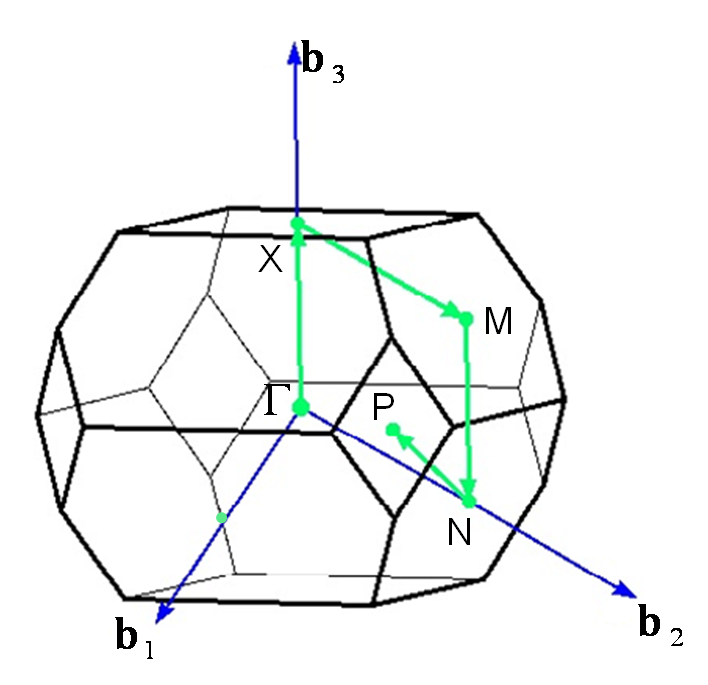
\includegraphics[height=50mm]{bz.eps}
\caption{The first Brillouin zone of CIGS}
\label{bz}
\end{center}
\end{figure}

\noindent The first Brillouin Zone (BZ) is the Wigner-Seitz primitive cell in reciprocal space, for example, the figure \ref{bz} is the first BZ of CIGS, where $\textbf{b}_1$, 
$\textbf{b}_2$ and $\textbf{b}_3$ are reciprocal lattice basis vectors. The following is the table about high symmetry points of the first BZ.


%\FloatBarrier
\vspace{10cm}


\begin{table}{}
\begin{center}
\begin{tabular}{|c|c|c|c|}
  \hline
  \multicolumn{4}{ | r |}{Points Coordinates($\textbf{b}_1$,$\textbf{b}_2$,$\textbf{b}_3$)} \\
  \hline
  $\Gamma$ & 0 & 0 & 0 \\
    \hline
   X & 0 & 0 & 1/2 \\
   \hline
   M & 0 & 1/2 & 1/2 \\
   \hline
   N & 0 & 1/2 & 0 \\
   \hline
   P & 1/2 & 1/2 & 1/2 \\
  \hline
\end{tabular}
\caption{\textit{High Symmetry Points of BZ for CIGS}}
\end{center}
\end{table}



\section{Band structure and density of state}
\noindent In solid, there are huge amount of atoms which interact each other, so the discrete of energy split into the huge number of state
 with small difference, those are defined as energy band, it is very important if one wants to know more about electrons or optical
 properties. So the band structure of CIGS is given as follows:

\begin{figure}[h]\label{bs}
\begin{center}
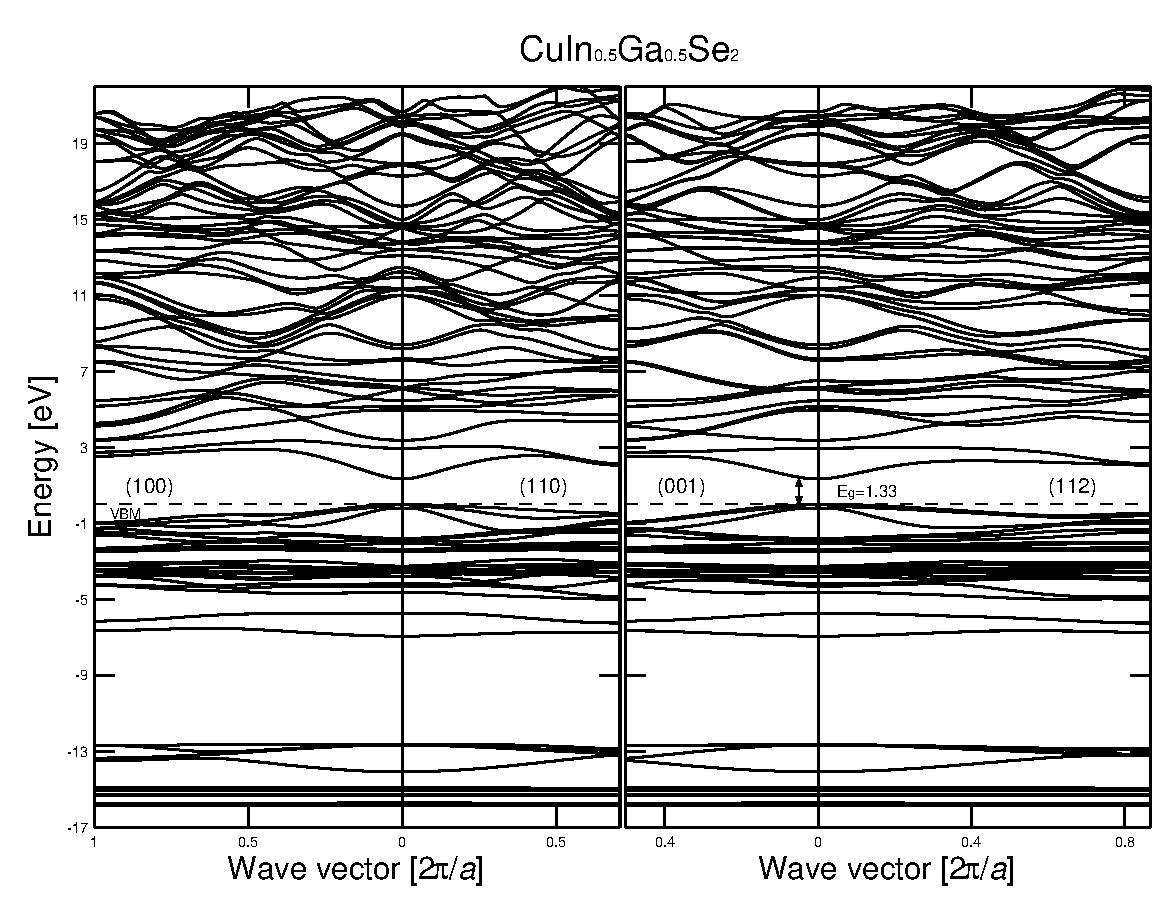
\includegraphics[height=90mm, width=110mm]{bandstr_theis.eps}
\caption{The band structure of CIGS}
\end{center}
\end{figure}

\noindent The density of states (DOS) of a system is the number of states which could be occupied per interval of energy. And the DOS of CIS is: 

\begin{figure}[h]\label{doscis}
\begin{center}
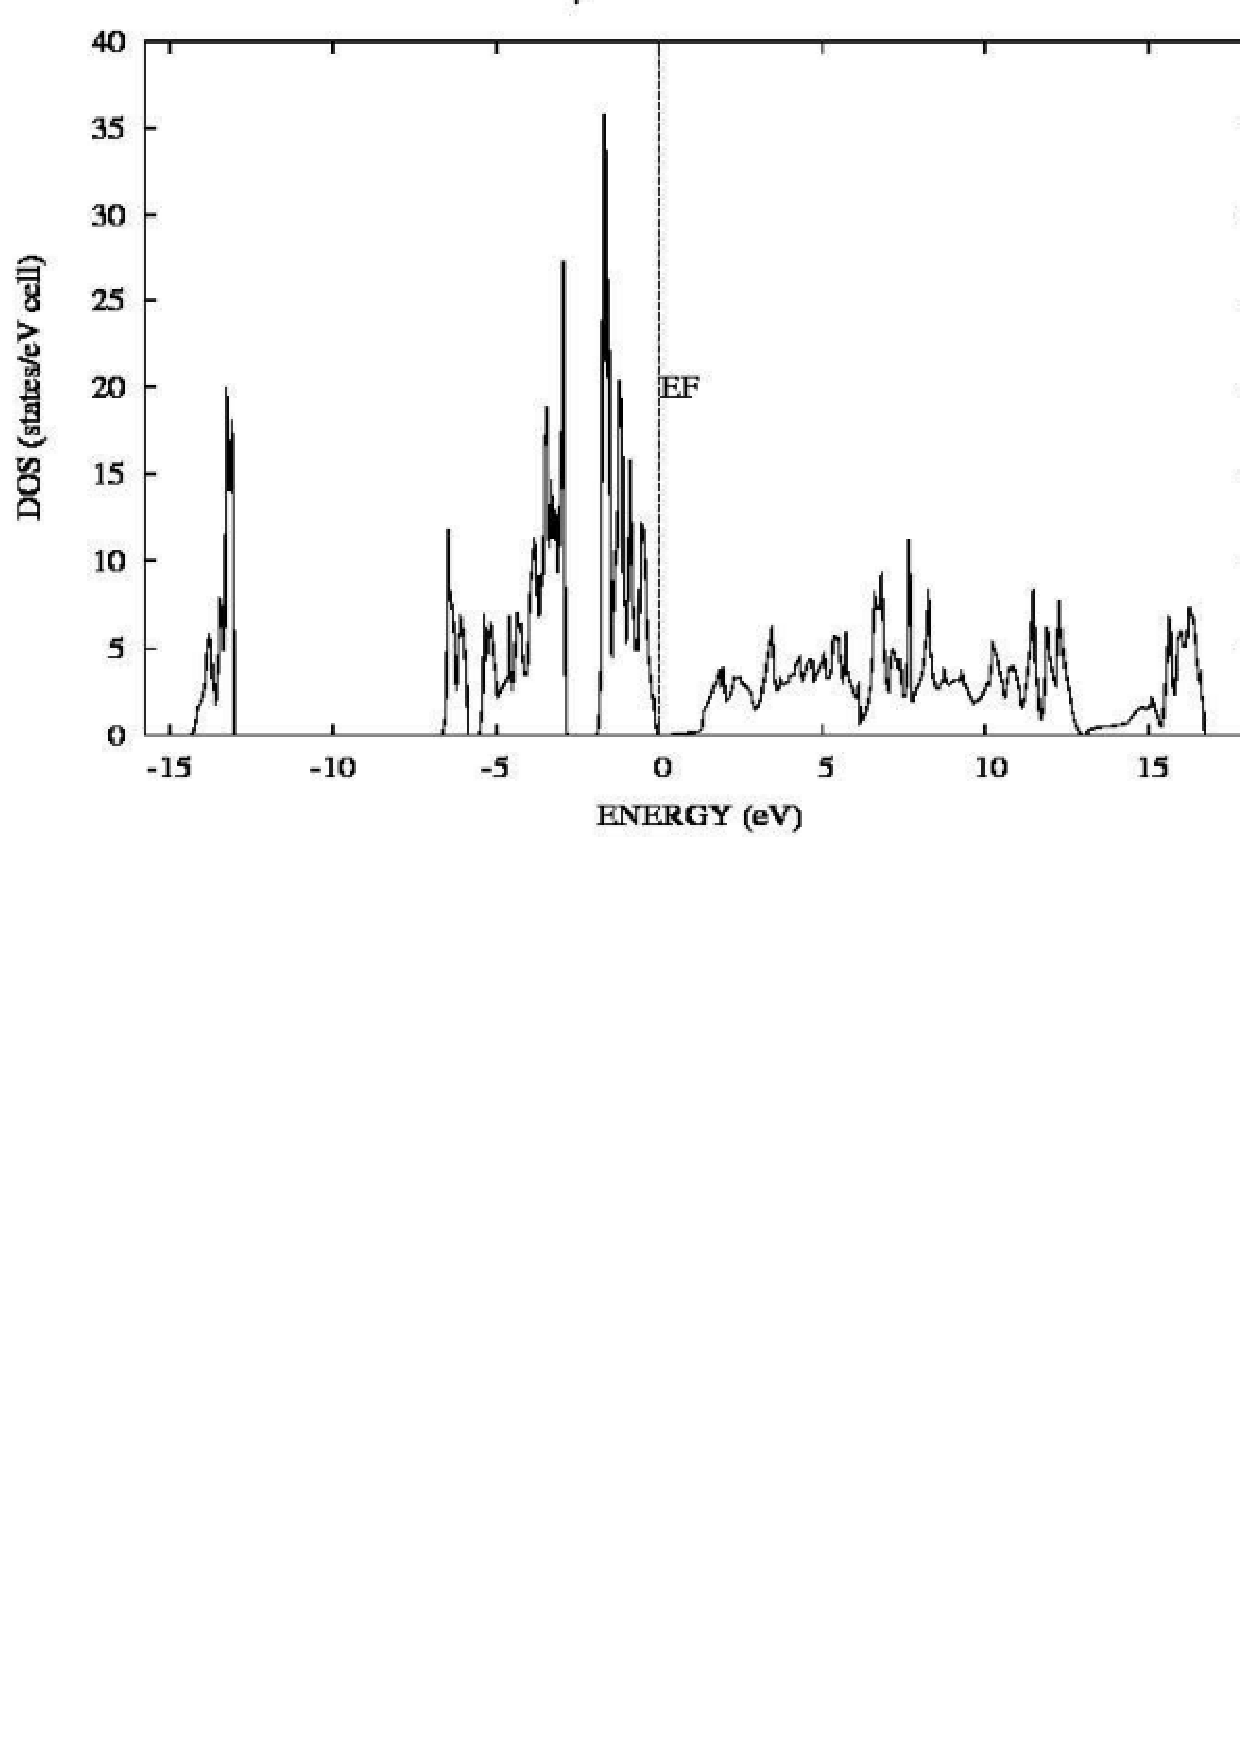
\includegraphics[scale=0.4]{doscis.png}
\caption{The band structure of CIS}
\end{center}
\end{figure}





\chapter{FP-LAPW method}
\section{Introduction}
\noindent So far, one already know how to solve the Kohn-Sham equation, however, there are still two more questions in the air, what is the exact form of 
wavefunction and potential in the realistical calculation?  

\noindent One maybe naturally choose the a set of plane waves as wavefunction because of bloch theory, but there is a drawback about the plane wave 
when describing the nearby the atomic core region, because the wavefunction change dramatically, so one needs to choose more plane
waves to define it, which means it will take more time to calculate.

\noindent Slater re-consider the way to describe the wavefunction, he splits the unit cell into two regions, one is the sphere region which is
defined by the center of atom, but non-overlap each sphere, called muffin tin (MT) region, the remaining region is called interstitial 
(I) region (see figure \ref{ucuc}). And an atomic like function is defined as the wavefunction in MT region, this is reason why the method is called augmented plane wave (APW),
 and in the interstitial region wavefunction is described as plane wave, which is reasonable, because the wave 
function approaching atomic core is somehow like inside atom, but far away the atomic core, the electron behaves like free electrons,
 so plane wave is suitable (see equation \ref{ap1}). However, the drawback of APW method is the wavefunction is dependent with the energy, which leads to the 
nonlinear eigenvalue problem (see equation \ref{ap2}), so in order to get the exact energy, the method have to decide repeatlly, which is really time-consumming.
%%%%%%%%%%%%%%%%% figure of mf and ir
\noindent In order to find a way out, is it possible to let the wavefunction energy-independent? Andesen, Koelling and Arbman propose a way to describe that,
they notice that the taylor expansion of radial function (see equation \ref{ap3}), and then make use of it to linearize the APW method, so the method is called Linearized Augmented Plane Wave (LAPW)
method. However, the drawback is that this method does not describe the semicore state well, so it is corrected by a method named LAPW+LO which is proposed by Singh (see equation \ref{lap1}). And
Sjöstedt, Nordström and Singh also give a efficient way to linearize Slater's APW method, named LAPW+lo (see equation \ref{lap3}).

%{\color{red}??????????????????? need to understant more about LAPW+LO and +lo ?????????????????????????} 


\section{Wavefunction}
\subsection{Augmented Plane Wave method}
\noindent Slater defines the wavefunction like the following equation:

%?????????????????????????????????????????????????????????????? comment here

\begin{equation}\label{ap1}
\phi^{APW}_{\textbf k+G} ({\textbf r})= 
\begin{cases} \frac {1}{\sqrt{\Omega}} e^{i({ \textbf k+G}) {\textbf r}} & \quad \mbox{if ${\textbf r} \in I, $} 
\\
\sumg<\alpha>\sum\limits_{{\ell}m} f_{{\ell}{m}} (r_{\alpha},{\textbf k+G}, E) Y_{{\ell}m}(\hat{{\textbf r}}_{\alpha})  & \quad \mbox{if $ {\textbf r} \in S_\alpha, $}\\ 
\end{cases}
\end{equation}





\noindent where $f_{{\ell}{m}} (r_{\alpha},\textbf{k+G} ,E) =  A _{{\ell}m}^{\alpha} \textbf(k+G) u_{{\ell}}^{\alpha}(r_{\alpha}, E)$ and $A _{{\ell}m}^{\alpha} \textbf(k+G) $is the expasion coefficients, and $u_{{\ell}}^{\alpha} (r_{\alpha}, E)$  is the radial function, which is dependent with energy $E$, and the
radial function could be decided by the following:


\begin{equation}\label{ap2}
(-\frac{1}{2} \frac{d^2}{dr_{\alpha}^2} + \frac{\ell(\ell+1)}{2r_{\alpha}^2}+V(r_{\alpha})-E)r_{\alpha}u_{\ell}(r_{\alpha}) = 0
\end{equation}


\noindent where $V(r_{\alpha})$ is the spherical potential.

%%%%%%%%%%%%%%%%%%%%%%  figure mt and interstial region

\noindent Because wavefunction has dual representations, one has to make sure the continousiny on the sphere, which is solved by matching each $\ell m$
of the dual representation.

\begin{figure}[h]
\begin{center}
\includegraphics[scale=0.7]{Presentation1.png}
\caption{Partition of the unit cell}
\label{ucuc}
\end{center}
\end{figure}


\noindent from the above figure, one will notice that the unit cell is divided into muffin-tin spheres ($\alpha$, $\beta$) and an
interstitial region (I), and ${\textbf r=R^{\alpha}+r_{\alpha}}$ is guaranted. so taking use of the Rayleigh expansion formula:

\begin{equation}
\expg<(k+G)>= e^{i \textbf(k+G) \textbf{R}^{\alpha} } 4 \pi \sumlm<\ell><m> i^{\ell} \bessf< |\textbf{k+G}|> \sphfr<\ell{m}><r><> \sphfq<\ell{m}><\textbf{k+G}><*>
\end{equation}
  
\noindent After matching those two representations, the following equation is satisfied:

\begin{equation}
A _{{\ell}m}^{\alpha} \textbf(k+G)= \frac{ e^{i \textbf(k+G) \textbf{R}^{\alpha} } 4 \pi \sumlm<\ell><m> i^{\ell} \bessf< |\textbf{k+G}|> \sphfq<\ell{m}><\textbf{k+G}><*> }{\sqrt{\Omega} u_{{\ell}}^{\alpha}(r_{\alpha}, E)}
\end{equation}

\noindent There are two main drawbacks about the APW method:
The first one is that the wavefuntion is energy dependent, which means that the code will search for the energy in order to calculate the exact energy, so it 
is really time consumming.The second one the less harmful, but also sometimes it will cause problem when $u_{{\ell}}^{\alpha}(r_{\alpha}, E) = 0$ during matching. 

\subsection{Linearized Augmented Plane Wave method}
\noindent In order to decouple the energy and wavefunction, Andesen, Koelling and Arbman find out a way to seperate them, they notice that the taylor expansion of the radial function
on certain energy, which can be expressed as follows:

\begin{equation}\label{ap3}
 u_{{\ell}}^{\alpha}(r_{\alpha}, E) = u_{{\ell}}^{\alpha}(r_{\alpha}, E_{\ell}) + (E-E_{\ell}) \dot{u}_{{\ell}}^{\alpha}(r_{\alpha}, E_{\ell})
\end{equation}

\noindent So they re-define the wavefuntion in the following way:

%?????????????????????????????????????????????????????????????? comment here

\begin{equation}\label{lap4}
\phi^{LAPW}_\textbf{k+G} (\textbf{r})= 
\begin{cases} \frac {1}{\sqrt{\Omega}} e^{i(\textbf{k+G})\textbf{r}} & \quad \mbox{if $\textbf{r} \in I, $}
\\
\sumg<\alpha>\sum\limits_{{\ell}m} f_{{\ell}{m}} (r_{\alpha},\textbf{k+G}, E_{\ell}) Y_{{\ell}m}(\hat{\textbf{r}}_{\alpha})  & \quad \mbox{if $\textbf{r} \in S_\alpha, $}\\ 
\end{cases}
\end{equation}


\noindent where $f_{{\ell}{m}} (r_{\alpha},\textbf{k+G} ,E_{\ell}) =  A _{{\ell}m}^{\alpha} \textbf(k+G) u_{{\ell}}^{\alpha}(r_{\alpha}, E_{\ell}) + B _{{\ell}m}^{\alpha} \textbf(k+G) \dot{u}_{{\ell}}^{\alpha}(r_{\alpha}, E_{\ell})$
, $A _{{\ell}m}^{\alpha} \textbf(k+G)$ and $B _{{\ell}m}^{\alpha} \textbf(k+G)$ are the expansion coefficients, and $\dot{u}_{{\ell}}^{\alpha}(r_{\alpha}, E_{\ell} )$ is the derivate of the radial function.

\noindent Here energy $E_{\ell}$  is considered as pre-calculated parameter, actually, it is chosen by the middle of  each $\ell$-character band.

\noindent Apparently, LAPW method is more suitable in reality, because the wavefunction is decoupled with energy, but it has to match for two parameters,
fortunately, even though, it still use less time comparing with APW method. However, there is one drawbacks, what if energy difference is bigger in the same $ {\ell} $ charater, 
which the $E_{\ell}$ is correct? so this situation will cause big error, these states are called as semi-core state, for example,the actinides and the rare earths and so on.

\subsection{Linearized Augmented Plane Wave method + LO}
Comparing with LAPW method, LAPW+LO method extend the basis set, and add smaller number of basis set, which has the following format:


\begin{equation*}\label{lap1}
\phi^{LO}_\textbf{k+G} (\textbf{r})= 
\begin{cases} 0 & \quad \mbox{if $\textbf{r} \in I, $}
\\
(A _{{\ell}m}^{\alpha}  u_{{\ell}}^{\alpha}(r_{\alpha}, E_{\ell}) + B _{{\ell}m}^{\alpha}  \dot{u}_{{\ell}}^{\alpha}(r_{\alpha}, E_{\ell}) + C _{{\ell}m}^{\alpha}  u_{{\ell}}^{\alpha}(r_{\alpha}, E^{\prime}_{\ell})){Y_{{\ell}m}(\hat{\textbf{r}}_{\alpha})} & \quad \mbox{if $\textbf{r} \in S_\alpha, $}\\ 
\end{cases}
\end{equation*}
 
\noindent where $A _{{\ell}m}^{\alpha}$ and $B _{{\ell}m}^{\alpha}$ is matching value and derivate on the sphere boundary to zero, but not plane wave, like LAPW did before, and $E^{\prime}_{\ell}$ is
the chosen energy from semi-core state.

\subsection{Augmented Plane Wave method plus local orbitals}
\noindent Actually, there is one more method which will deal with the energy-denpendent case, which is called as Augmented Plane Wave method plus local orbitals (APW+lo), the 
basis function has two kinds, one is similar with equation \ref{lap1}, but only without the derivative terms, e.g., $f_{{\ell}{m}} (r_{\alpha},\textbf{k+G} ,E_{\ell}) =  A _{{\ell}m}^{\alpha} \textbf(k+G) u_{{\ell}}^{\alpha}(r_{\alpha}, E_{\ell})$.
And another basis function is:
\begin{equation*}\label{lap3}
\phi^{lo}_\textbf{k+G} (\textbf{r})= 
\begin{cases} 0 & \quad \mbox{if $\textbf{r} \in I, $}
\\
(A _{{\ell}m,lo}^{\alpha}  u_{{\ell}}^{\alpha}(r_{\alpha}, E_{\ell}) + B _{{\ell}m,lo}^{\alpha}  \dot{u}_{{\ell}}^{\alpha}(r_{\alpha}, E_{\ell}) ){Y_{{\ell}m}(\hat{\textbf{r}}_{\alpha})} & \quad \mbox{if $\textbf{r} \in S_\alpha, $}\\ 
\end{cases}
\end{equation*}
 
\noindent And the value of $A _{{\ell}m,lo}^{\alpha}$ and $B _{{\ell}m,lo}^{\alpha}$ are obtained by normalization and local orbital has zero value at the muffin tin boundary.


\section{Potential}

The potential in the FP-LAPW method is also divided into two regions, one is in the MT region, another one is in the interstital region.
\begin{equation*}\label{lap3}
V(\textbf{r})= 
\begin{cases} \sumg<{\textbf G}> V_{\textbf G} e^{i {\textbf G} {\textbf {r}  }} & \quad \mbox{if $\textbf{r} \in I, $}
\\
 \sum\limits_{{\ell}m} V_{{\ell}m}^{\alpha} (r_{\alpha}) Y_{{\ell}m}(\hat{{\textbf r}}_{\alpha})  & \quad \mbox{if $\textbf{r} \in S_\alpha, $}\\ 
\end{cases}
\end{equation*}


\chapter{K $\cdot$ P method}

%%%%%%modify the sentences below


The band dispersion can be obtained exactly by using the kp method in principle, the basic idea will be explained in the following text.

First, if the Schrödinger equation is defined as follows:

\begin{equation}\label{kpse}
\left\{ \frac {{\textbf p}^2} {2m} + V({\textbf r}) \right\} \wfbloch<n><k> = \ebloch<n><k> \wfbloch<n><k>
\end{equation}

where ${\textbf p} = i \hbar \bigtriangledown $ and the Bloch theory shows:

\begin{equation}\label{1}
 \wfbloch<n><k> = \expg<k> \ubloch<n><k>
\end{equation}

where $\wfbloch<n><k>$ is the wave function on ${\textbf k}$ point for the {$\textit n$}th band, and $\expg<k>$ is plane wave, $\ubloch<n><k>$ is a function which has the same a periodicity as the potential.

If substituting the equation \ref{1} to \ref{kpse}, it will end up the following equation:

\begin{equation}
 \{  \frac{{\textbf p}^2}{2m} + V({\textbf r }) + \frac{{\hbar^2 {\textbf k}^2}}{2m} + \frac{{\hbar \textbf {kp}}}{m} \} \ubloch<n><k>  =  \ebloch<n><k> \ubloch<n><k>
\end{equation}

In the above equation, if $\textbf k = 0$, then the Hamiltonian turn out to be $H_0 = {\textbf p}^2 / {2m} + V({\textbf r })$, so here the first two terms are treated as unpertubation term, and pertubation term is seen as
$W={{\hbar^2 {\textbf k}^2}}/{2m} + {{\hbar \textbf {kp}}}/{m}$, the result will be as follows after treating the equation as pertubation.

\begin{equation}
 \ebloch<n><k> = E_{n,0} + \frac{{\hbar^2 {\textbf k}^2}}{2m} + \frac{ \hbar^2}{m^2} \suminj<i><j> \frac{|<\ubloch<n><0>|{\textbf {kp}}|\ubloch<n'><0>>|^2}{E_{n,0} - E_{n',0}}
\end{equation}


Now let us suppose the wavefunction and energy are obtained by some procedures on $k_0$ point, $\wfbloch<n><k_0>$ is the wavefunction and $\ebloch<n><k_0>$ is the energy.
And another function is defined as follows:

\begin{equation}\label{2}
\chikp<n><k> = \expg<(k-k_0)>  \wfbloch<n><k_0> 
\end{equation}

The above function $\chikp<n><k> $ is expanded as wave function on ${ \textbf k}$ point, and then the wave function on the ${\textbf k}$ point is calculated by:
\begin{equation}\label{3}
\wfbloch<n><k> =  {\sum\limits_{j}} C_{n,j}^{k} \chikp<j><k> 
\end{equation}

From above equation, the wave function is known if the coefficient $C_{n,j}^{k}$ is obtained, let us substitute the equation \ref{3} into Kohn-Sham equation \ref{kpse}.
Finally the following equation is obtained:

\begin{equation}\label{5}
{\sum\limits_{j}}  C_{n,j}^{k} \left \{  \left [  \ebloch<j><k_0> -  \ebloch<n><k>  + \frac{{\hbar}^2}{2m} {\textbf (k^2-k_0^2)}    \right ] \delta_{j',j} + \frac{\hbar}{m} {\textbf(k-k_0)} {\textbf p_{j',j}} \right \} = 0
\end{equation}

where ${\textbf p_{j',j}} = \langle \ubloch<j'><k_0>| {\textbf p} | \ubloch<j><k_0>  \rangle $.
 
We also can simpify the above equation in the following format:
\begin{equation}\label{6}
{\sum\limits_{j}} C_{n,j}^{k} \left \{ H_{j',j}- \ebloch<n><k> \delta_{j',j} \right \} =0
\end{equation}

where
\begin{equation} \label{7}
H_{j',j} = \left [  \ebloch<j><k_0>  + \frac{{\hbar}^2}{2m} {\textbf (k^2-k_0^2)}    \right ] \delta_{j',j} + \frac{\hbar}{m} {\textbf(k-k_0)} {\textbf p_{j',j}}
\end{equation}

From the above equation, the coefficient $ C_{n,j}^{k}$ is calculated.


\begin{comment}
Actually, if substituting the equation \ref{1} into equation \ref{4}, the analytical expression of band dispersion can be obtained.
 \begin{equation} \begin{split}\label{8}
& \ebloch<n><k> {\expg<k> \ubloch<n><k>} = \left\{ \frac {{\textbf p}^2} {2m} + V({\textbf r}) \right\} {\expg<k> \ubloch<n><k>} \\
& = \expg<k> \left \{ \frac {{\textbf p}^2} {2m} + V({\textbf r}) +  \frac {{\textbf k}^2 \hbar^2 } {2m}  + \frac { \hbar {\textbf k \cdot p}} {m}  \right\} \ubloch<n><k>
\end{split}
\end{equation} 

so 
 \begin{equation} \label{9}
\ebloch<n><k> {\ubloch<n><k>} = \left \{ \frac {{\textbf p}^2} {2m} + V({\textbf r}) +  \frac {{\textbf k}^2 \hbar^2 } {2m}  + \frac { \hbar {\textbf k \cdot p}} {m}  \right\} \ubloch<n><k>
\end{equation} 
\end{comment}


%t\chapter{CIGS material}
%discribe from Si to CIGS, bonding, and so on


\chapter{Result and discussion}

\section{Parameterization of energy bands for $\cigs$}
In this section, first the parameterization of energy bands (three uppermost valence bands and the lowest conduction band) is described, and then in order to demonstrate
the anisotropic and non-parabolic of energy bands, some properties are investigated, such as effective electron and hole masses, constant energy surface and so on.
To explain the importance of this parameterization, the density-of-states, Fermi energy and carrier concentrations are analyaed and compared.

The following figure shows the fitting result from the parameterization of energy bands for $\cigs$, right column subfigure shows the closed up of right column subfigure.
In this figure, the energies are referred to the VBM (dashed lines). Spin-orbit coupling is included, however, the notation of the energy bands (j = v1, v2, v3, and c1) 
refers to a spin-independent band indexing where c1 represents the lowest CB and v1 represents the topmost VB; The solid lines show the full-potential
 results from ?? and ??, the circles are the results of the full band parameterization from Ref. ??, and the dotted lines represent the parabolic band approximation.
one can notice that the parabolic bands describe the two uppermost VBs poorly in the directions (100), (110), and (112), and the parameterized energy bands can describe the energy bands around 0.5 eV
below the VBM and around 0.5 eV above the CB minimum (CBM). 

\begin{figure}[H]
\begin{center}$
\begin{array}{cc}
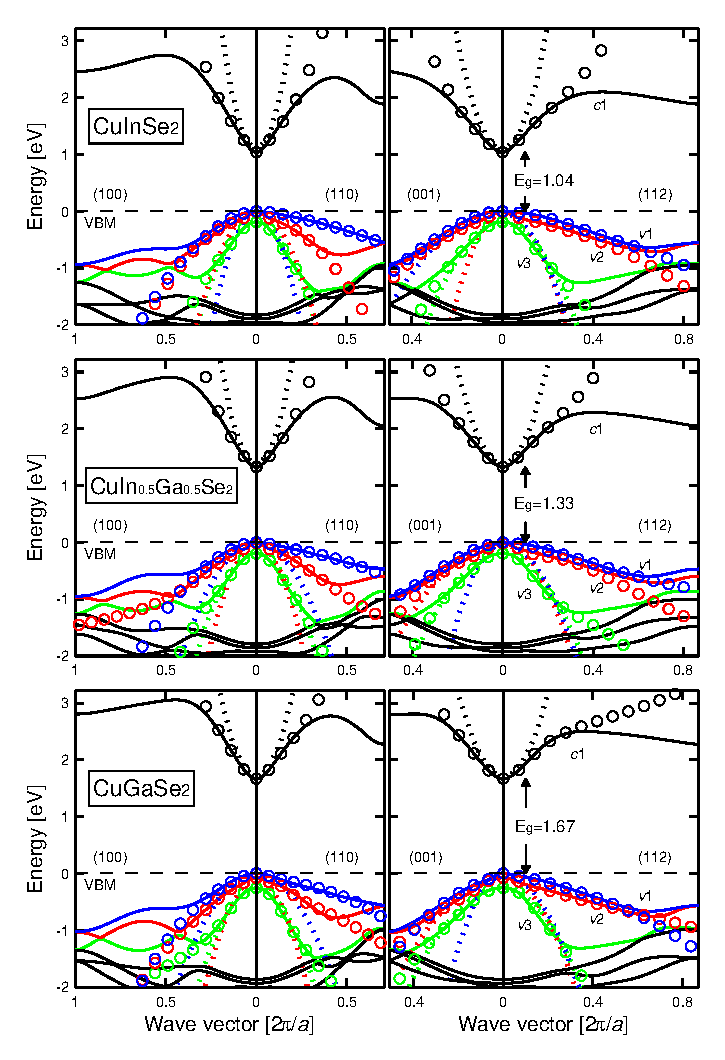
\includegraphics[scale=.6]{paper2figure1.eps} &
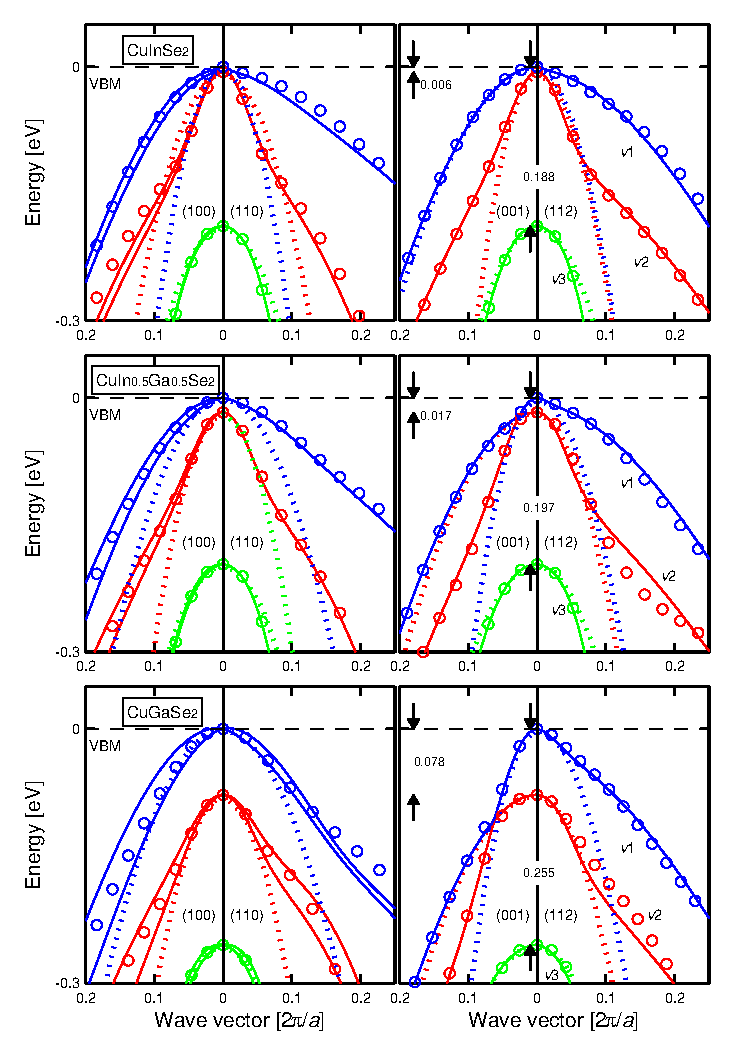
\includegraphics[scale=.6]{paper2figure2.eps}
\end{array}$
\end{center}
\caption{Electronic band structure $E_j({\textbf k})$ of $\mathrm {CuInSe_2}$  (upper panels),  $\mathrm {CuIn_{0.5}Ga_{0.5}Se_2}$  (middle panels), and $\mathrm {CuGaSe_2}$ (lower panels) along four directions}
\label{paper2figure1}
\end{figure}

To further more illustrate the parameterization of energy bands, the effective electron and hole mass tensors are determined along the four symmetry directions in the 
following figure. The figure shows that the effective hole masses of the two topmost VBs show very strong anitotropy at the $\Gamma$ point, however, the CB has a rather isotropic electron mass tensor at the $\Gamma$
point.

\begin{figure}[H]
\begin{center}
\includegraphics[scale=.6]{paper1figure3.eps} 
\end{center}
\caption{Inverse of the effective electron and hole masses for $\cigs$ (x = 0, 0.5, and 1) in the four symmetry directions, obtained from the second derivative of the energy dispersion:
 $m_j(\textbf{k}))^{-1} = \pm (\partial^2 E_j(\textbf{k})/{\partial{\textbf{k}}^2})/\hbar^2. $ }
\end{figure}

And here is the figure of constant energy surface of $\mathrm {CuIn_{0.5}Ga_{0.5}Se_2}$, which demonstrates that the VBs and CB have ellipsoidal shapes in the vicinity of the $\Gamma$-point,
but that they are very non-parabolic and anisotropic away from the $\Gamma$-point, as well as corresponding results for $\mathrm {CuInSe_2}$ and $\mathrm {CuGaSe_2}$.
  
\begin{figure}[H]
\begin{center}
\includegraphics[scale=.6]{cigs_sm.eps}
\end{center}
\caption{Constant energy surfaces $S_j(E)$ for the three uppermost VBs and the lowest conduction band in $\mathrm {CuIn_{0.5}Ga_{0.5}Se_2}$ for the energies E = 1 meV  and E = 200 meV. }
\end{figure}

The total DOS of the VBs and CB are presented in the following figure, which demonstrates that the non-parabolicity of the bands strongly affect the DOS dispersions
and the difference between parabolic approximation and the parameterization of the bands is remarkable. In the figure, the solid lines show the full band 
parameterization (fbp), and the dashed lines represent the parabolic band approximation (pba). The parameterization always generates larger DOS, this is
corresponding to the parameterization result of overall band curvature is flatter than the one at the nearby VBM and CBM.

\begin{figure}[H]
\begin{center}
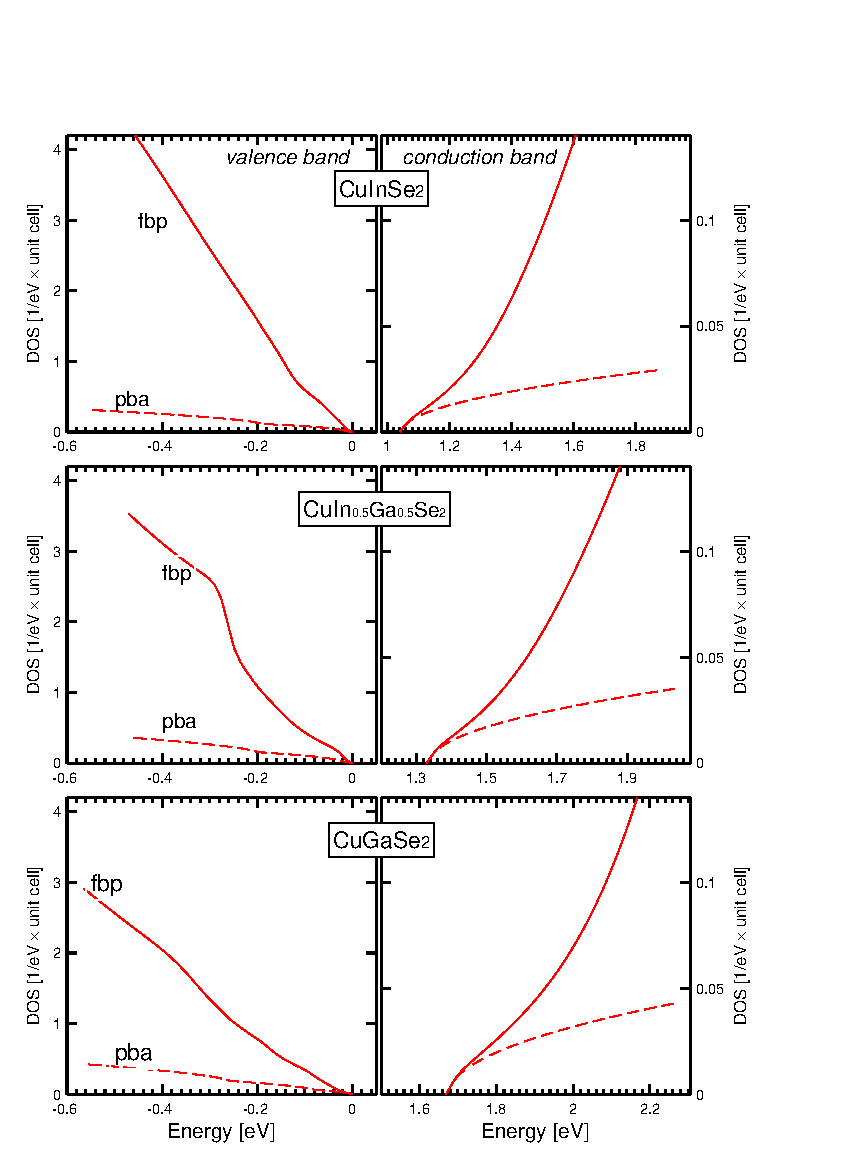
\includegraphics[scale=.6]{paper2figure4.eps}
\end{center}
\caption{Total DOS of the VBs (left panels) and of the CB (right panels) for $\mathrm {CuInSe_2}$, $\mathrm {CuIn_{0.5}Ga_{0.5}Se_2}$, and $\mathrm {CuGaSe_2}$.  }
\end{figure}

From the total DOS and from the constant energy surfaces, the number of states with energies up to E is determined (Fig. \ref{paper2figure5}). This quantity describes thus the carrier
concentration due to external band filling of holes in the VBs and electrons in the CB for the given quasi-Fermi energies $E_{F,v*}$ and $E_{F,c*}$, respectively, and at
temperature T = 0 K. In agreement with the discussion above for the total DOS, it is obvious that the VBs (CB) in Ga rich compounds will be less (more) populate
by holes (electrons) for a given quasi-Fermi energy $E_{F,v*}$ ($E_{F,c*}$). Thus, CuGaSe2 can more easily host free electrons due to a more flat CB. However, a flat band 
implies heavier mass and thereby a weaker response to an applied electric field, which is negative for the electron transport.  
Fig. \ref{paper2figure5} also demonstrates that the parabolic approximation of the bands strongly underestimates the band filling in the VBs and the CB. For example, the number of
VB states of $\mathrm {CuInSe_2}$ is increased by a factor of $\sim$18 at the positive energy $|\bigtriangleup E| = E_{v1}(\textbf 0) - E_{F,v*}$ = 0.1 eV when the non-parabolicity is included, and for the
corresponding CB the number is increased by a factor of $\sim$3. At $|\bigtriangleup E|$ = 0.5 eV, the increase is as much as $\sim$41 and $\sim$8 times, respectively. This will have a strong
impact on modeling band filling of especially holes for p-type $\cigs$ materials.

\begin{figure}[H]
\begin{center}
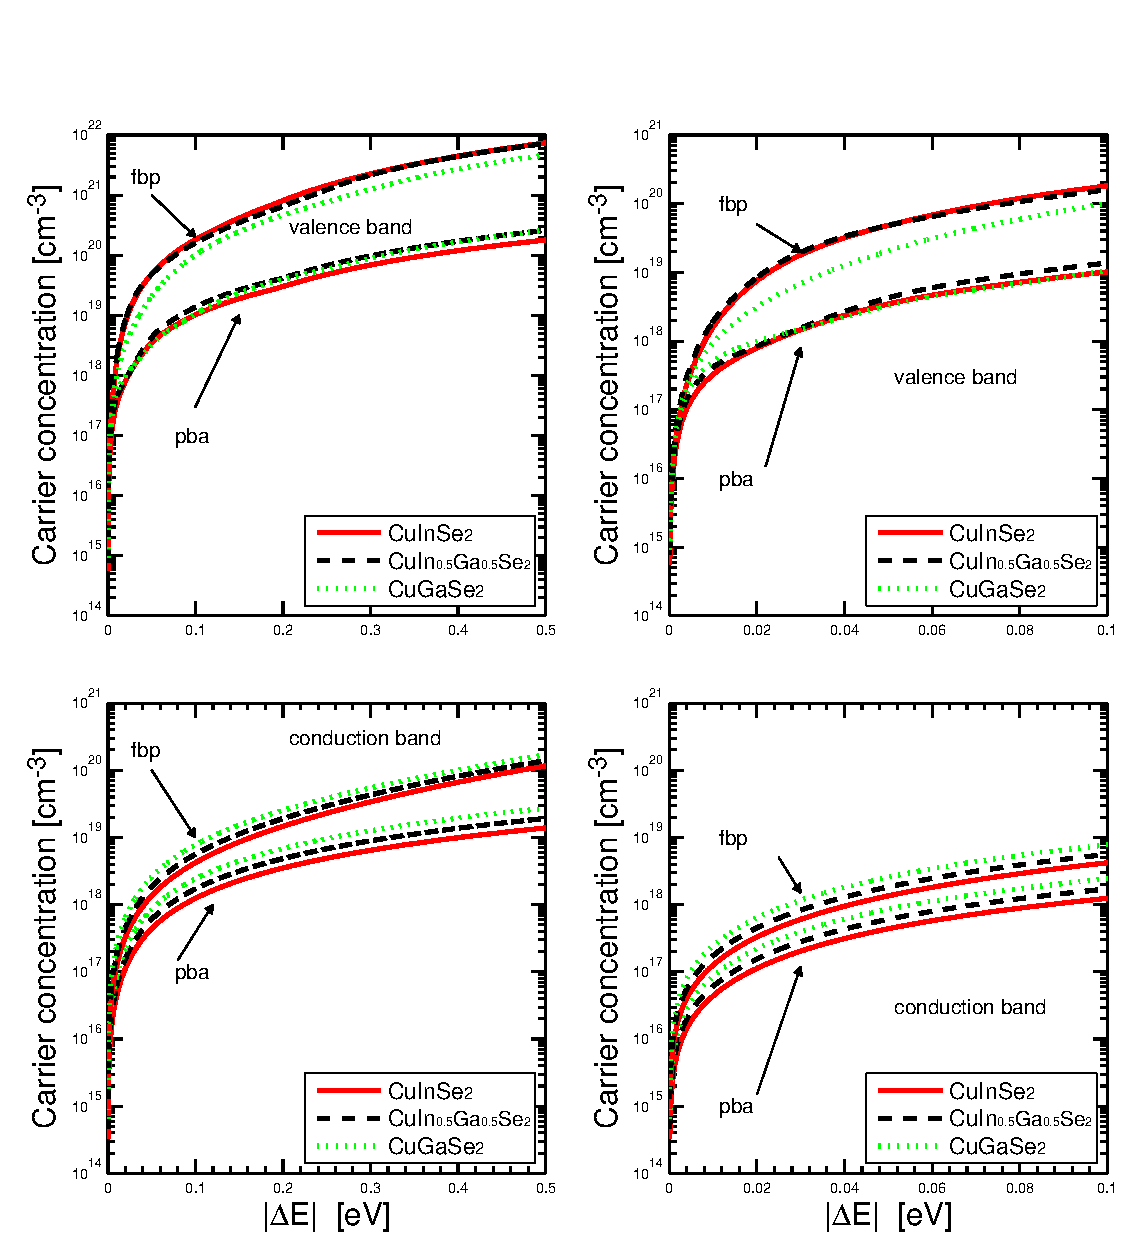
\includegraphics[scale=.6]{paper2figure5.eps}
\end{center}
\caption{ Carrier concentration p or n as functions of the quasi-Fermi energy $E_F^*$ of the VBs $E_{F,v*}$ and of the CB $E_{F,c*}$. 
left column shows the results for large energy scale up to 0.5 eV, and right column displays a close-up for small Fermi energies. 
In the figure, $|\bigtriangleup E|$ is the positive energy difference $E_{v1}(\textbf 0) - E_{F,v*}$ for the VBs and $E_{F,c*} - E_{c1}(\textbf 0)$ for the CB. 
The carrier concentrations consider external band filling in intrinsic materials at T = 0 K. The results demonstrate that the parabolic band approximation strongly
underestimates the band filling of both the VBs and CB. }
\label{paper2figure5}
\end{figure}


The DOS masses for the $\cigs$ (Fig. \ref{paper2figure6}) show a very strong energy dependence of the VB DOS mass. This is directly related to the non-parabolicity and anisotropy
of the VBs (cf. Fig. \ref{paper2figure1} ). For instance, the VB DOS masses in $\mathrm {CuInSe_2}$ is $m_{v1}(E \approx 0) = (m^{\perp}_{v1}m^{\perp}_{v1}m^{\parallel}_{v1})^{1/3} = 0.23m0$ in the vicinity of the $Gamma$-point. This mass increases to $\sim$1.00m0 when
E is increased to $\sim$0.1 eV. This may therefore explain the large measured hole masses $m_{v1} \approx 0.7m0$ in $\mathrm {CuInSe_2}$ (Refs. ?? and ??) and $\sim$0.64m0 in $\mathrm {CuGaSe_2}$ (Ref. ??) since
indirect measurements normally involves high hole concentrations.

The absolute change in the CB DOS mass is small, but the relative increase is 2 to 3 times with respect to the $\Gamma$-point value:  = 0.080m0, 0.103m0, and 0.130m0, 
whereas = 0.234m0, 0.255m0, and 0.316m0, for $\mathrm {CuInSe_2}$, $\mathrm {CuIn_{0.5}Ga_{0.5}Se_2}$, and $\mathrm {CuGaSe_2}$, respectively.

\begin{figure}[H]
\begin{center}
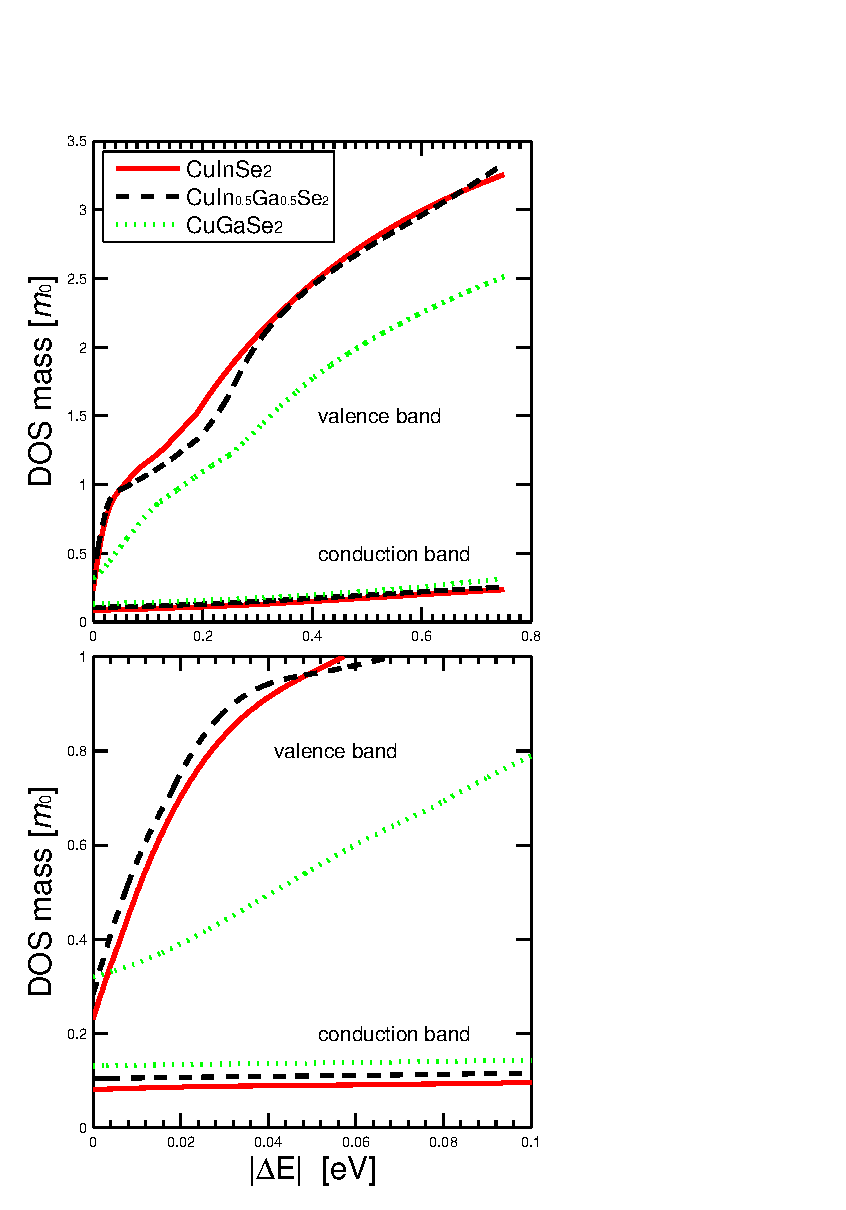
\includegraphics[scale=.6]{paper2figure6.eps}
\end{center}
\caption{The DOS mass of the VBs and the CB in $\mathrm {CuInSe_2}$, $\mathrm {CuIn_{0.5}Ga_{0.5}Se_2}$, and $\mathrm {CuGaSe_2}$. The upper (lower) panel shows  in a wider (narrower) energy region. 
This energy-dependent mass generates accurate quasi-Fermi energy $E_{F,v*}$ and $E_{F,c*}$ as function of the carrier concentration; $|\bigtriangleup E|$ is the energy difference 
 $E_{v1}(\textbf 0) - E_{F,v*}$ for the VBs and $E_{F,c*} - E_{c1}(\textbf 0)$ for the CB; cf.  Fig. \ref{paper2figure5}  }
\label{paper2figure6}
\end{figure}





The band gap and the Fermi level of intrinsic $\mathrm {CuIn_{0.5}Ga_{0.5}Se_2}$ are presented in the following figure.At temperature $T \approx 0 K$ the band gap is
$E_g(0)$ = 1.04, 1.33, and 1.67 eV for x = 0, 0.5, and 1, respectively, and the Fermi level is exactly the mid-gap energy $E_F(0) = E_g(0)/2$. With increasing temperature,
the band gap is decreased. The corresponding Fermi level changes only slightly with temperature, but for $\mathrm {CuInSe_2}$ and $\mathrm {CuIn_{0.5}Ga_{0.5}Se_2}$, the Fermi levels increase
somewhat more compared with $\mathrm {CuGaSe_2}$. This is primarily due to the CB of DOS mass for $\mathrm {CuGaSe_2}$ is almost the same, but the VB of DOS mass for $\mathrm {CuGaSe_2}$ change smaller
compared with CuInSe2 and CuIn0.5Ga0.5Se2 which will affect the DOS. As a consequence, the Fermi level is closer to the CB minimum in the In rich compounds. 
At T = 300 K and 600 K the band-gap energies and Fermi energy are $E_g(300)$ = 1.02, 1.29, and 1.62 eV, $E_g(600)$ = 0.98, 1.24, and 1.55 eV, $E_F(300)$ = 0.55, 0.69,
and 0.84 eV, and $E_F(600)$ = 0.59, 0.71, and 0.84 eV for x = 0, 0.5, and 1 respectively. The largest effect is thus seen for the Ga rich compounds,
however the temperature effect is rather moderate.

\begin{figure}[H]
\begin{center}
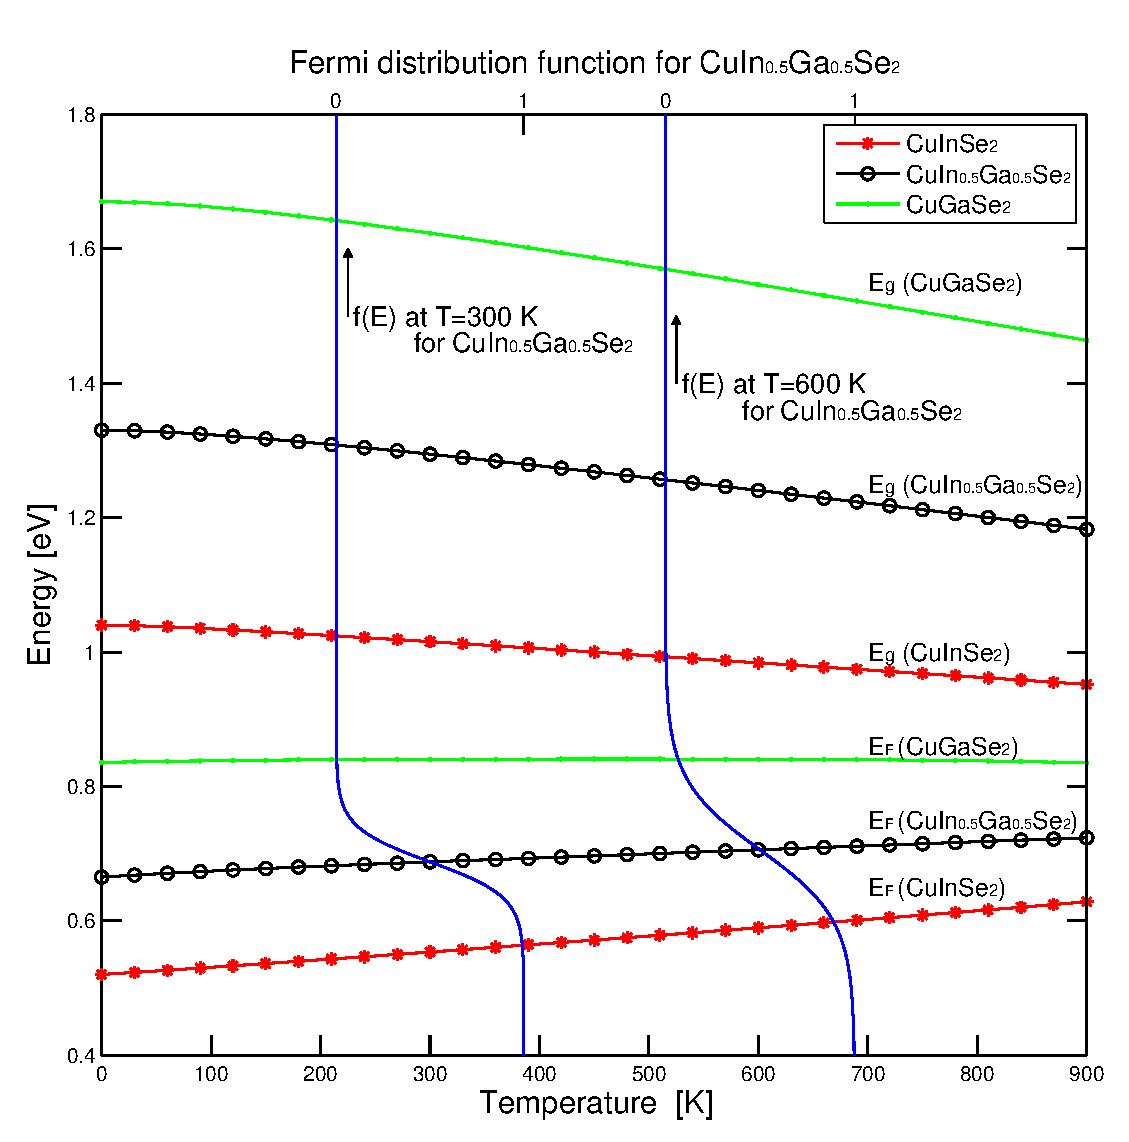
\includegraphics[scale=.6]{paper2figure7a_1.eps}
\end{center}
\caption{Band-gap energy $E_g$ and Fermi energy $E_F$ for $1 \leq  T \leq 900 K$ of intrinsic  $\mathrm {CuInSe_2}$, $\mathrm {CuIn_{0.5}Ga_{0.5}Se_2}$, and $\mathrm {CuGaSe_2}$, 
determined from the full band parameterization. In this figure, he Fermi distribution f(E) of $\mathrm {CuIn_{0.5}Ga_{0.5}Se_2}$ is presented for T = 300 K and 600 K as well.}
\label{paper2figure7a}
\end{figure}


The calculated Fermi level  in p-type materials is presented in the following figure, referred to the Fermi level of the intrinsic materials $E_F$ from figure
\label{paper2figure7a}. Only at very high temperatures ($T > 400 K$) and for low acceptor concentrations, the Fermi level of p-type $\cigs$
will reach the Fermi level of corresponding intrinsic compounds. Moreover, although the different compounds have comparable acceptor ionization energies, 
the Ga rich alloy has lower relative Fermi level; this is a direct consequence of the larger band gap of the Ga rich alloy. By comparing the calculations with
the parabolic band approximation  (dotted lines in Fig. \ref{paper2figure7a}) and the full band approach (solid lines) for each of the three $\cigs$ alloys,
one can notice that the Femi level is similar for the two models only at low and at very high temperatures. In the mid-temperature region the difference is 
however apparent, especially for the high acceptor concentrations. Assuming parabolic bands yields always a lower Fermi level. The reason for this effect is 
that the energy dependent effective mass  in the full band parameterization is always larger that the corresponding $\Gamma$-point mass. Although the effect on the
 absolute value of the Fermi level seems to be small, it has an impact on the free carrier concentrations for highly doped materials.


\begin{figure}[H]
\begin{center}
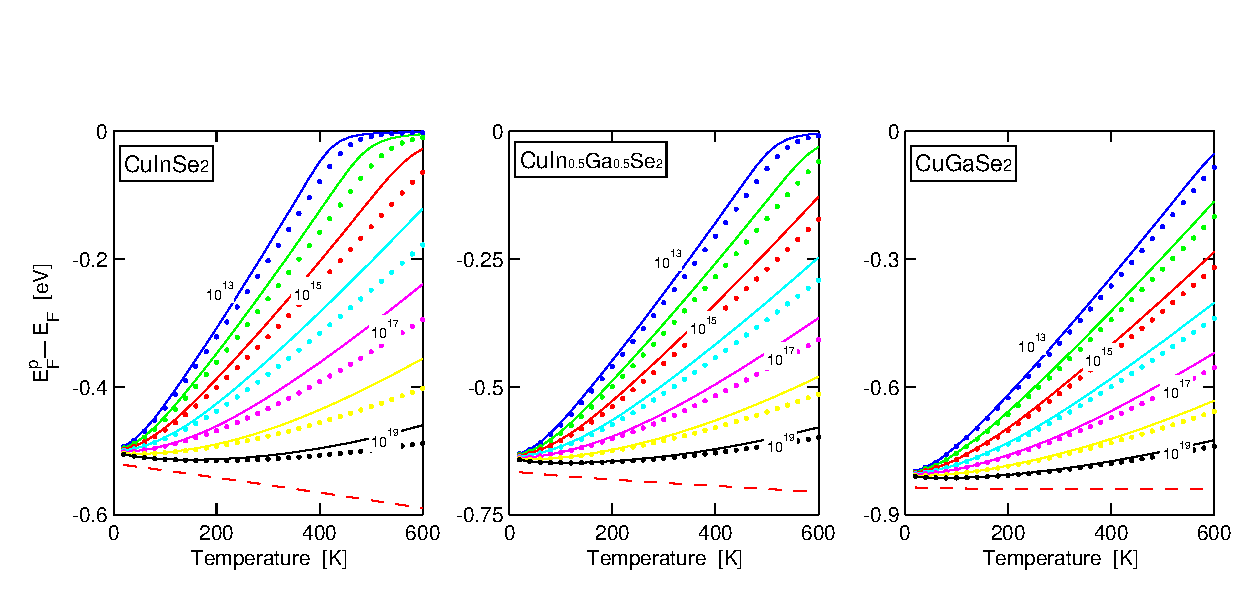
\includegraphics[scale=.6]{paper2figure8.eps}
\end{center}
\caption{Fermi level as function of the temperature $20\leq T \leq600$ of p-type $\mathrm {CuInSe_2}$, $\mathrm {CuIn_{0.5}Ga_{0.5}Se_2}$, and $\mathrm {CuGaSe_2}$ for the effective doping concentration 
$N_A = 10^{13}, 10^{14},10^{15}, …,$ and $10^{19}$  acceptors/$cm^3$. The energy scale $E_F^p - E_F$ describes the Fermi energy with respect to the
intrinsic $E_F$; see Fig. \ref{paper2figure7a}. Dashed lines represent the VBM with respect to the intrinsic Fermi level. Solid and dotted lines represents the full band parameterization and the parabolic band approximation,
 respectively.}
\label{paper2figure8}
\end{figure}

The free carrier concentrations of p-type $\cigs$ as functions of temperature and acceptor concentration are presented in the following figure. The carrier concentration
 can be divided into three regions: the freeze-out region for low temperatures, the extrinsic region in the mid-temperature region, and the intrinsic region at
 sufficiently high temperatures. For example, consider $\mathrm {CuInSe_2}$ with the acceptor concentration $N_A = 10^{13} cm^3$ . At very low temperatures ($T < 100 K$), 
part of the host electrons are excited to the acceptor-like states whereas remaining host electrons are “frozen”. With an increase of the temperature, more and more
 electrons in the VBs are thermally excited, until all acceptor states are occupied. The calculated concentrations in this region are in fairly good agreement with 
experimental carrier concentrations from low-temperature Hall mobility measurements by Schroeder et al.9  Both the calculated and measured data indicate that the 
freeze-out region is as high as room-temperature even for moderately doped $\mathrm {CuInSe_2}$ ( $N_A \approx 10^{17}$ to $10^{18}$  $cm^3 $). 
With a further increase of the temperature, the free carrier concentration will be constant for a wide temperature range; this is the extrinsic region.
 When the temperature is increase even further, the free carrier concentration will be enhanced due to electron excitation across the band gap as for 
the intrinsic materials.

\begin{figure}[H]
\begin{center}
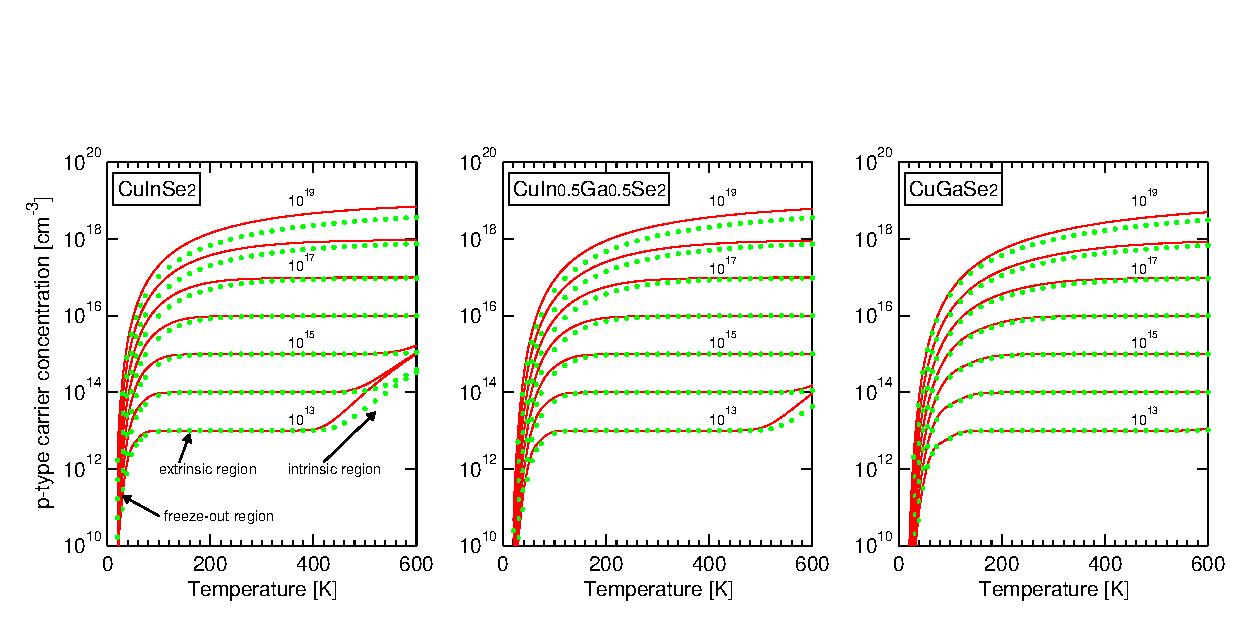
\includegraphics[scale=.6]{paper2figure9.eps}
\end{center}
\caption{ Free carrier concentration as function of the temperature in p-type $\mathrm {CuInSe_2}$, $\mathrm {CuIn_{0.5}Ga_{0.5}Se_2}$, and $\mathrm {CuGaSe_2}$ for the effective doping concentration
 $N_A = 10^{13}, 10^{14}, 10^{15}, …,$ and $10^{19}$ acceptors/$cm^3$. Solid and dotted lines represents the full band parameterization and the parabolic band approximation,
 respectively. The full band description of the energy dispersion is important for high doping concentrations and/or in the intrinsic region for cross-gap
 excitations at high temperatures. }
\label{paper2figure9}
\end{figure}

From the above figure, one can observe that the transition from the freeze-out region to the extrinsic region occurs well below the room temperature unless
the uncompensated acceptor concentration is above $~10^{18} cm^3$. Due to the slightly lower ionization energies for the In rich compounds, these compounds 
have lower temperature for the transition to the extrinsic region. For high uncompensated acceptor concentrations (i. e., $>10^{18} cm^3$) not all acceptors 
are ionized at room temperature (see Table $I$). Moreover, since the In rich compounds also have smaller band gaps, the transition from the extrinsic 
region to the intrinsic region occurs at lower temperatures for these compounds. The intrinsic region is however only important for very low acceptor 
concentrations. 

By comparing the results from the parabolic band approximation and from the full band parameterization for each compound, one can observe that the 
approximation underestimates the free carrier concentrations roughly by a factor of 2 in both the freeze-out region and also in the intrinsic regions.
Due to this underestimate, the transition from freeze-out to extrinsic regions tends to occur at a somewhat higher temperature for the approximated method,
and also the transition from the extrinsic to the intrinsic region also at a somewhat higher temperature. Although the carrier concentration is fully described 
in the extrinsic region by assuming parabolic bands since all acceptors are ionized, the Fermi level is not well described within this approximation (see Fig. \ref{paper2figure8}). 
Thus, in order accurately describe the free carrier concentration as well as its temperature dependency, a full description of the energy dispersions is needed. 




To summarize, the energy band dispersion and the carrier concentration in chalcopyrite $\cigs$ (x = 0, 0.5, and 1) alloys is analyzed. 
The overall results are: i) the three uppermost VB are strongly anisotropic and non-parabolic. (ii) The lowest CB becomes non-parabolic for energies 50-100 meV
above the $\Gamma$-point band minimum. (iii) A constant DOS mass cannot accurately describe band filling of the VBs even at low hole concentrations. Instead, 
an energy dependent DOS mass is introduced that can be utilized to describe the carrier concentration and the Fermi energy using traditional equations for the DOS.
(iv) With the full description of the energy dispersion, the hole concentration is improved by a factor of 10–50 and the electron concentration is improved by a 
factor of 2–10 depending on quasi-Fermi energy.  (v) The transition from the freeze-out region to the extrinsic region occurs well below the room temperature for
 uncompensated acceptor concentration below $~10^{17} cm^3$, whereas for higher concentrations not all acceptors are ionized at T = 300 K. 
Thus, with a more correct description of the energy dispersions, one can better analyze the electron and hole dynamics in the $\cigs$ alloys, thereby better understand the electrical properties of these compounds.  


\section{Dielectric function spectra of $\mathrm {CuIn_{0.5}Ga_{0.5}Se_2}$ }
In this section, first the $\varepsilon$ spectra of $\mathrm {CuIn_{0.5}Ga_{0.5}Se_2}$ which is calculated by FPLAPW method is described and compared with experiment
result, and then different contributions to $\varepsilon_2$ in terms of the transitions between the valence bands and the conduction bands are identified, at last, 
the $\textbf{k}$-dependence of the CPs along the main symmetry directions is analyzed. 


Real ($\varepsilon_1$) and imaginary ($\varepsilon_2$) parts of the modeled $\varepsilon$ spectra for $\mathrm {CuIn_{0.7}Ga_{0.3}Se_2}$ taken at 40 and 300 K are given in the following
figure(a).The overall shape of the SE-determined $\varepsilon$ data shows a good agreement with the averaged $\varepsilon=[2\varepsilon_\perp+\varepsilon_\parallel]/3$ spectrum for $\mathrm {CuIn_{0.5}Ga_{0.5}Se_2}$ 
calculated by the FPLAPW method with the GGA+U potential that is presented in the following figure(b). Although the Ga/(Ga+In) ratio x for the experimental data
 (x=0.3) and calculated spectrum (x=0.5) are different, our calculations suggest that no significant difference in the optical properties is anticipated 
between those two close compositions, other than the shift of CP energies. This is also evidenced by the similarities in the calculated $\varepsilon$ spectrum and the CP 
features between $\mathrm {CuIn_{0.5}Ga_{0.5}Se_2}$ and $\mathrm {CuInSe_2}$.

\begin{figure}[H]
\begin{center}
\includegraphics[scale=.15]{paper3figure1.png}
\end{center}
\caption{ (a) Modeled $\varepsilon_1$ and $\varepsilon_2$ spectra for $\mathrm {CuIn_{0.7}Ga_{0.3}Se_2}$ 
 taken at 40 K (solid blue lines) and 300 K (dashed red lines).
 Four prominent above-bandgap CP features are indicated by arrows, which are labeled in the numeric and alphabetic order. 
 (b) The $\varepsilon$ spectra for $\mathrm {CuIn_{0.5}Ga_{0.5}Se_2}$
 calculated by the FPLAPW using the GGA + U. The majob CP features corresponding to the SE results are identified. }
\label{paper3figure1}
\end{figure} 


The electronic origins of each CP are examined based on the results from the FPLAPW calculations. First, the different contributions to $\varepsilon_2$ is identified in terms of
 the transitions between the valence bands $v_i$ and the conduction bands $c_j$. Here, the $v_1$ and $c_1$ denote the highest valence band and lowest conduction band, 
respectively. This contribution is labeled as $v1 \leftrightarrow c1$ in the following figure. As expected,8,9 the $E_0$ CPs in the low-energy region are associated with the transitions from v1 
to c1 near the $\Gamma$ (0, 0, 0) point of the Brillouin zone (BZ). A broad optical structure in the $\varepsilon_2$ spectrum spanning from 5 to 7 eV is composed of several contributions
 from the low-lying valence bands. Therefore, unambiguous identification of the major contributions to the CP features in the high-energy region is very difficult.

\begin{figure}[H]
\begin{center}
\includegraphics[scale=.8]{paper3figure2.eps}
\end{center}
\caption{ Band-to-band analysis of the contribution to the total $\varepsilon_2$ spectrum (thin black trace). The most important valence-to-conduction band transitions $v_i \leftrightarrow c_j$) 
are marked by thick colored curves. Spin-orbit interaction is included, and the band-to-band transitions involve a summation of the spin up and down contributions.
 Note: The vertical axis $\varepsilon_2$ is in the log scale.}
\label{paper3figure2}
\end{figure} 


The ${\textbf k}$-dependence of the CPs along the main symmetry directions is analyzed , which is depicted in the following figure. The pronounced $E_1$ CP originates from the$v_1 \leftrightarrow c_1$ transitions
 near the $P (1/2,1/2, 1/2)$ point of the BZ (in the conventional coordinates). This is consistent with the results from room-temperature SE studies by Alonso et al.,$??8,??9$ 
where this CP is assigned to the $E_1$(A) CP. We observed a small doublet structure in the $E_1$ peak arising from the spin-orbit split. The $E_2$ and $E_3$ CPs involve
 transitions from the second valence band, $v2 \longrightarrow c1$. This band-to-band transition generates two structures in $\varepsilon_2$, where the main peak is associated with transitions 
at the P-point as for the $E_1$ CP. In $\mathrm {CuIn_{0.5}Ga_{0.5}Se_2}$, the $E_2$ and $E_3$ peaks modify only slightly the main $\varepsilon_2$ spectrum around 3.2 eV. However, the calculations for 
$\mathrm {CuInSe_2}$ reveal that the $E_2$ and $E_3$ CPs occur 0.1 to 0.2 eV higher than the $E_1$ CP, and appear as distinct spectral features. Thus, the observation of $E_2$ and $E_3$ CPs in 
$\mathrm {CuIn_{0.7}Ga_{0.3}Se_2}$  is anticipated. The $E_4$ CP originates from the $v3 \longrightarrow c1$ transitions at the $M (1,0,0) = M* (0,0,1)$ point. The $E_5$ CP is mainly attributed to the 
transition to $v4 \longrightarrow c1$ at the $N (1/2, 0, 1/2)$ point, but the $v3 \longrightarrow c1$ transitions at the $M/M^*$ points also contribute to this CP feature. This $E_5$ CP can be understood as
 the $E_1$(B) CP in previous SE studies.$??8,??9$ The $E_6$ CP feature is a result of the $v4 \longrightarrow c1$ transition at the N point. The $E_7$ CP corresponds to the $v4 \longrightarrow c2$ transitions at
 the $\Gamma$ (0, 0, 0) and N point, and the $v5 \longrightarrow c2$ transitions at the $\Gamma$ point. The EA, another prominent CP feature equivalent to the $E_2$(A) CP in Refs. $??8,??9$, also has
 multiple contributions from the various symmetric points of BZ: The $v1 \longrightarrow c4$ transitions at the $X^* (1/2, 1/2, 0)$ point of the BZ, and the $v1 \longrightarrow c3$ transitions at the N
 and P points. We conjecture that the $v11 \longrightarrow c1$ and $v12 \longrightarrow c1$ transitions near the P point of BZ are the major contributions to the $E_C$ CP. Although this CP has not
 been discussed in previous SE studies $??8,??9$ of $\cigs$ probably due their limit on the spectral range, a recent real-time SE study $??12$ of $\mathrm {CuInSe_2}$ observed a similar
 structure at 5.11 eV without identification of its electronic origin.


\begin{figure}[H]
\begin{center}
\includegraphics[scale=.8]{paper3figure3.eps}
\end{center}
\caption{The calculated electronic band structure of $\mathrm {CuIn_{0.5}Ga_{0.5}Se_2}$ where the CPs are identified along the main symmetry directions. Contributions of individual CPs to the $\varepsilon_2$ are shown in Fig. \ref{paper3figure2}}
\label{paper3figure3}
\end{figure} 




In summary, the  $\varepsilon$ spectra for $\mathrm {CuIn_{0.7}Ga_{0.3}Se_2}$ were determined by spectroscopic ellipsometry at 40 and 300 K. From a standard lineshape analysis of ellipsometric data,
 a total of twelve CP energies were obtained from 2.5 to 6.4 eV, which include two additional CPs at 3.01 and 3.48 eV. Electronic origins of the observed CP features
 were discussed based on the results from FPLAPW calculations of the electronic band structure for $\mathrm {CuIn_{0.5}Ga_{0.5}Se_2}$ . The pairs of valence and conduction bands along 
the main symmetry directions of Brillouin zone were suggested for the major CP features observed in the $\varepsilon_2$ spectra.
\end{document}
